\flushbottom



%%
%% Add a section on the difference differential equation.
%%








%%=============================================================================
%%=============================================================================
\chapter{The Laplace Transform}



%%=============================================================================
\section{The Laplace Transform}
\index{Laplace transforms}


The Laplace transform of the function $f(t)$ is defined
\[
\mathcal{L}[f(t)] = \int_0^\infty \e^{-s t} f(t)\,\dd t,
\]
for all values of $s$ for which the integral exists.
The Laplace transform of $f(t)$ is a function of $s$ which we will
denote $\hat{f}(s)$.
\footnote{Denoting the Laplace transform of $f(t)$ 
  as $F(s)$ is also common.}


A function $f(t)$ is of exponential order $\alpha$ if there exist constants
$t_0$ and $M$ such that 
\[ 
|f(t)| < M \e^{\alpha t}, \quad \mathrm{for all}\ t > t_0.
\]

If $\int_0^{t_0} f(t)\,\dd t$ exists 
and $f(t)$ is of exponential order $\alpha$ then the Laplace transform $\hat{f}(s)$
exists for $\Re(s) > \alpha$.

Here are a few examples of these concepts.
\begin{itemize}
\item $\sin t$ is of exponential order $0$.
\item $t \e^{2 t}$ is of exponential order $\alpha$ for any $\alpha > 2$.
\item $\e^{t^2}$ is not of exponential order $\alpha$ for any $\alpha$.
\item $t^n$ is of exponential order $\alpha$ for any $\alpha > 0$.
\item $t^{-2}$ does not have a Laplace transform as the integral diverges.
\end{itemize}




\begin{Example}
  Consider the Laplace transform of $f(t) = 1$.
  Since $f(t) = 1$ is of exponential order $\alpha$ for any $\alpha > 0$,
  the Laplace transform integral converges for $\Re(s) > 0$.
  \begin{align*}
    \hat{f}(s)    
    &= \int_0^\infty \e^{-s t}\,\dd t \\
    &= \left[-\frac{1}{s} \e^{-s t}\right]_0^\infty \\
    &= \frac{1}{s}
  \end{align*}
\end{Example}








\begin{Example}
  The function $f(t) = t \e^t$ is of exponential order $\alpha$ for any
  $\alpha > 1$.  We compute the Laplace transform of this function.
  \begin{align*}
    \hat{f}(s)    
    &= \int_0^\infty \e^{-s t} t \e^{t}\,\dd t \\
    &= \int_0^\infty t \e^{(1-s)t}\,\dd t \\
    &= \left[\frac{1}{1-s} t \e^{(1-s)t}\right]_0^\infty - 
    \int_0^\infty \frac{1}{1-s}\e^{(1-s)t}\,\dd t \\
    &= -\left[\frac{1}{(1-s)^2}\e^{(1-s)t}\right]_0^\infty \\
    &= \frac{1}{(1-s)^2} \quad \mathrm{for}\ \Re(s) > 1.
  \end{align*}
\end{Example}








\begin{Example}
  Consider the Laplace transform of the Heaviside function,
  \[
  H(t-c) = \begin{cases}
    0\quad &\mathrm{for}\ t < c \\
    1\quad &\mathrm{for}\ t > c,
  \end{cases}
  \]
  where $c>0$.
  \begin{align*}
    \mathcal{L}[H(t-c)]
    &= \int_0^\infty \e^{-s t} H(t-c)\,\dd t \\
    &= \int_c^\infty \e^{-s t}\,\dd t \\
    &= \left[\frac{\e^{-s t}}{-s}\right]_c^\infty \\
    &= \frac{\e^{-c s}}{s} \quad \mathrm{for}\ \Re(s) > 0
  \end{align*}
\end{Example}







\begin{Example}
  Next consider $H(t-c)f(t-c)$.
  \begin{align*}
    \mathcal{L}[H(t-c)f(t-c)]
    &= \int_0^\infty \e^{-s t} H(t-c)f(t-c)\,\dd t \\
    &= \int_c^\infty \e^{-s t} f(t-c)\,\dd t \\
    &= \int_0^\infty \e^{-s (t+c)} f(t)\,\dd t \\
    &= \e^{-c s} \hat{f}(s)
  \end{align*}
\end{Example}






%%=============================================================================
\section{The Inverse Laplace Transform}
\index{Laplace transform!inverse}


The \textit{inverse Laplace transform} in denoted
\[
f(t) = \mathcal{L}^{-1}[\hat{f}(s)].
\]
We compute the inverse Laplace transform with
the \textit{Mellin inversion formula}.
\index{Mellin inversion formula}
\[ 
f(t) = \frac{1}{\imath 2 \pi} \int_{\alpha - \imath \infty}^{\alpha + \imath \infty} \e^{s t} \hat{f}(s)\,\dd s
\]
Here $\alpha$ is a real constant that is to the right of the 
singularities of $\hat{f}(s)$.

To see why the Mellin inversion formula is correct, we take the Laplace 
transform of it.  Assume that $f(t)$ is of exponential order $\alpha$.
Then $\alpha$ will be to the right of the singularities of $\hat{f}(s)$.
\begin{align*}
  \mathcal{L}[\mathcal{L}^{-1}[\hat{f}(s)]] 
  &= \mathcal{L}\left[\frac{1}{\imath 2 \pi} \int_{\alpha - \imath \infty}^{\alpha + \imath \infty} 
    \e^{z t} \hat{f}(z)\,\dd z \right] \\
  &= \int_0^\infty \e^{-s t} \frac{1}{\imath 2 \pi} \int_{\alpha - \imath \infty}^{\alpha + \imath \infty} 
  \e^{z t} \hat{f}(z)\,\dd z\,\dd t \\
  \intertext{We interchange the order of integration.}
  &= \frac{1}{\imath 2 \pi} \int_{\alpha - \imath \infty}^{\alpha + \imath \infty} \hat{f}(z) \int_0^\infty \e^{(z-s)t}\,\dd t\,\dd z \\
  \intertext{Since $\Re(z) = \alpha$, the integral in $t$ exists for $\Re(s) > \alpha$.}
  &= \frac{1}{\imath 2 \pi} \int_{\alpha - \imath \infty}^{\alpha + \imath \infty} \frac{\hat{f}(z)}{s-z}\,\dd z 
\end{align*}
We would like to evaluate this integral by closing the path of integration 
with a semi-circle of radius $R$ in the right half plane and applying the
residue theorem.  However, in order for the integral along the semi-circle 
to vanish as $R \to \infty$, $\hat{f}(z)$ must vanish as $|z| \to \infty$.  
If $\hat{f}(z)$ vanishes we can use the maximum modulus bound to show that 
the integral along the semi-circle vanishes.  
This we assume that $\hat{f}(z)$ vanishes at infinity.


Consider the integral,
\[
\frac{1}{\imath 2 \pi} \oint_C \frac{\hat{f}(z)}{s-z}\,\dd z,
\]
where $C$ is the contour that starts at $\alpha - \imath R$, goes straight up
to $\alpha + \imath R$, and then follows a semi-circle back down to 
$\alpha - \imath R$.  This contour is shown in Figure~\ref{contour}.

\begin{figure}[h!]
  \begin{center}
    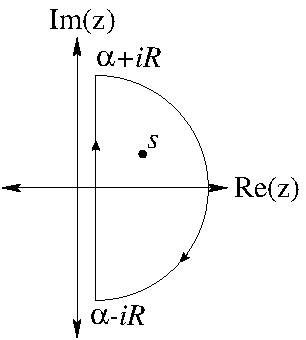
\includegraphics[width=0.25\textwidth]{ode/laplace/proof}
  \end{center}
  \caption{The Laplace transform pair contour.}
  \label{contour}
\end{figure}






If $s$ is inside the contour then
\[
\frac{1}{\imath 2 \pi} \oint_C \frac{\hat{f}(z)}{s-z}\,\dd z = \hat{f}(s).
\]
Note that the contour is traversed in the negative direction.  Since
$\hat{f}(z)$ decays as $|z| \to \infty$, the semicircular contribution to the
integral will vanish as $R \to \infty$.  Thus
\[
\frac{1}{\imath 2 \pi} \int_{\alpha - \imath \infty}^{\alpha + \imath \infty} \frac{\hat{f}(z)}{s-z}\,\dd z = \hat{f}(s).
\]
Therefore, we have shown than 
\[
\mathcal{L}[\mathcal{L}^{-1}[\hat{f}(s)]] = \hat{f}(s).
\]

$f(t)$ and $\hat{f}(s)$ are known as Laplace transform pairs.
\index{Laplace transform pairs}





%%-----------------------------------------------------------------------------
\subsection{$\hat{f}(s)$ with Poles}


%% CONTINUE
%% Also do for t < 0.
\begin{Example}
  Consider the inverse Laplace transform of $1/s^2$.  
  $s=1$ is to the right of the singularity of $1/s^2$.
  \[
  \mathcal{L}^{-1}\left[ \frac{1}{s^2} \right]
  = \frac{1}{\imath 2 \pi} \int_{1 - \imath \infty}^{1 + \imath \infty} \e^{s t} \frac{1}{s^2} \,\dd s 
  \]
  Let $B_R$ be the contour starting at $1 - \imath R$ and following a straight line
  to $1 + \imath R$;
  let $C_R$ be the contour starting at $1 + \imath R$ and following a semicircular
  path down to $1 - \imath R$.
  Let $C$ be the combination of $B_R$ and $C_R$.
  This contour is shown in Figure~\ref{bromwich1}. 


  \begin{figure}[h!]
    \begin{center}
        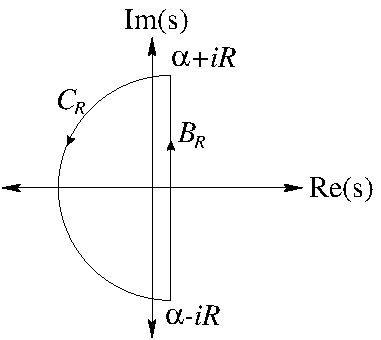
\includegraphics[width=0.3\textwidth]{ode/laplace/ooss}
      \caption{The path of integration for the inverse Laplace transform.}
      \label{bromwich1}
    \end{center}
  \end{figure}


  Consider the line integral on $C$ for $R > 1$.
  \begin{align*}
    \frac{1}{\imath 2 \pi}\oint_C \e^{s t} \frac{1}{s^2}\,\dd s
    &= \Res\left( \e^{s t} \frac{1}{s^2}, 0 \right) \\
    &= \frac{\dd}{\dd s} \e^{s t}\Big|_{s=0} \\
    &= t
  \end{align*}
  If $t \geq 0$, the integral along $C_R$ vanishes as $R \to \infty$.
  We parameterize $s$.
  \begin{gather*}
    s = 1 + R \e^{\imath \theta}, \qquad \frac{\pi}{2} \leq \theta \leq \frac{3\pi}{2} \\
    \big| \e^{s t} \big| = \left| \e^{t(1 + R \e^{\imath \theta})} \right|
    = \e^t \e^{t R \cos \theta} \leq \e^t
  \end{gather*}
  \begin{align*}
    \left|\int_{C_R} \e^{s t} \frac{1}{s^2}\,\dd s \right|
    &\leq \int_{C_R} \left| \e^{s t} \frac{1}{s^2}\right| \,\dd s \\
    &\leq \pi R \e^t \frac{1}{(R-1)^2} \\
    &\to 0\ \mathrm{as}\ R \to \infty
  \end{align*}

  Thus the inverse Laplace transform of $1/s^2$ is
  \[ 
  \boxed{
    \mathcal{L}^{-1}\left[\frac{1}{s^2}\right] = t, 
    \quad \mathrm{for}\ t \geq 0.
    }
  \]
\end{Example}







Let $\hat{f}(s)$ be analytic except for isolated poles at $s_1, s_2, \ldots,s_N$ and
let $\alpha$ be to the right of these poles.  Also, let $\hat{f}(s) \to 0$ as 
$|s| \to \infty$.  Define $B_R$ to be the straight line from $\alpha - \imath R$
to $\alpha + \imath R$ and $C_R$ to be the semicircular path from
$\alpha + \imath R$ to $\alpha - \imath R$.  If $R$ is large enough to 
enclose all the poles, then
\begin{gather*} 
  \frac{1}{\imath 2 \pi} \oint_{B_R+C_R} \e^{s t} \hat{f}(s)\,\dd s 
  = \sum_{n=1}^N \Res(\e^{s t} \hat{f}(s), s_n) 
  \\
  \frac{1}{\imath 2 \pi} \int_{B_R} \e^{s t} \hat{f}(s)\,\dd s 
  = \sum_{n=1}^N \Res(\e^{s t} \hat{f}(s), s_n)
  - \frac{1}{\imath 2 \pi} \int_{C_R} \e^{s t} \hat{f}(s)\,\dd s.
\end{gather*}

Now let's examine the integral along $C_R$.  Let the maximum of $|\hat{f}(s)|$
on $C_R$ be $M_R$.  We can parameterize the contour with
$s = \alpha + R\e^{\imath \theta}$, $\pi/2 < \theta < 3\pi/2$.
\begin{align*}
  \left| \int_{C_R} \e^{s t} \hat{f}(s)\,\dd s \right|
  &= \left| \int_{\pi/2}^{3\pi/2} \e^{t(\alpha + R\e^{i\theta})}
    \hat{f}(\alpha + R\e^{\imath \theta}) R \imath \e^{\imath \theta}\,\dd \theta \right| \\
  &\leq \int_{\pi/2}^{3\pi/2} \e^{\alpha t} \e^{t R \cos \theta} R M_R \,\dd \theta \\
  &= R M_R \e^{\alpha t} \int_0^\pi \e^{-t R \sin \theta}\,\dd \theta \\
  \intertext{If $t \geq 0$ we can use Jordan's Lemma to obtain,}
  &< R M_R \e^{\alpha t} \frac{\pi}{t R}. \\
  &= M_R \e^{\alpha t} \frac{\pi}{t} \\
  \intertext{We use that $M_R \to 0$ as $R \to \infty$.}
  &\to 0 \quad \mathrm{as}\ R \to \infty
\end{align*}
Thus we have an expression for the inverse Laplace transform of $\hat{f}(s)$.
\begin{gather*}
  \frac{1}{\imath 2 \pi} \int_{\alpha - \imath \infty}^{\alpha + \imath \infty} \e^{s t} \hat{f}(s)\,\dd s = 
  \sum_{n=1}^N \Res(\e^{s t} \hat{f}(s), s_n) \\
  \mathcal{L}^{-1}[\hat{f}(s)] = \sum_{n=1}^N \Res(\e^{s t} \hat{f}(s), s_n)
\end{gather*}










\begin{Result}
  \label{Res_lt_poles}
  If $\hat{f}(s)$ is analytic except for poles at $s_1, s_2, \ldots, s_N$ and 
  $\hat{f}(s) \to 0$ as $|s| \to \infty$ then the inverse Laplace transform of 
  $\hat{f}(s)$ is
  \[ 
  f(t) = \mathcal{L}^{-1}[\hat{f}(s)] = \sum_{n=1}^N \Res(\e^{s t} \hat{f}(s), s_n), 
  \quad \mathrm{for}\ t > 0.
  \]
\end{Result}













\begin{Example}
  Consider the inverse Laplace transform of $\frac{1}{s^3 - s^2}$.

  First we factor the denominator.
  \[ 
  \frac{1}{s^3 - s^2} = \frac{1}{s^2} \frac{1}{s-1}. 
  \]
  Taking the inverse Laplace transform,
  \begin{align*}
    \mathcal{L}^{-1} \left[ \frac{1}{s^3-s^3} \right]
    &= \Res \left( \e^{s t} \frac{1}{s^2} \frac{1}{s-1}, 0 \right) + 
    \Res \left( \e^{s t} \frac{1}{s^2} \frac{1}{s-1}, 1 \right) \\
    &= \frac{\dd}{\dd s} \frac{\e^{s t}}{s-1}\bigg|_{s=0} + \e^t \\
    &= \frac{-1}{(-1)^2} + \frac{t}{-1} + \e^t 
  \end{align*}
  Thus we have that
  \[ 
  \boxed{
    \mathcal{L}^{-1}\left[\frac{1}{s^3-s^2} \right] = \e^t-t-1,
    \quad \mathrm{for}\ t > 0.
    }
  \]
\end{Example}







\begin{Example}
  Consider the inverse Laplace transform of
  \[ 
  \frac{s^2 + s - 1}{s^3 - 2s^2 + s - 2}.
  \]
  We factor the denominator.
  \[
  \frac{s^2 + s - 1}{(s - 2)(s - \imath)(s + \imath)}.
  \]
  Then we take the inverse Laplace transform.
  \begin{align*}
    \mathcal{L}^{-1}\left[\frac{s^2+s-1}{s^3-2s^2+s-2}\right]
    &= \Res\left( \e^{s t} \frac{s^2+s-1}{(s - 2)(s - \imath)(s + \imath)}, 2 \right)
    + \Res \left( \e^{s t} \frac{s^2+s-1}{(s - 2)(s - \imath)(s + \imath)}, \imath \right) \\
    &\qquad \qquad
    + \Res \left( \e^{s t} \frac{s^2+s-1}{(s - 2)(s - \imath)(s + \imath)}, -\imath \right) \\
    &= \e^{2t} + \e^{\imath t} \frac{1}{\imath 2} + \e^{-\imath t} \frac{-1}{\imath 2}
  \end{align*}
  Thus we have
  \[
  \boxed{
    \mathcal{L}^{-1}\left[\frac{s^2+s-1}{s^3-2s^2+s-2}\right]
    = \sin t + \e^{2t}, \quad \mathrm{for}\ t > 0.
    } 
  \]
\end{Example}









%%-----------------------------------------------------------------------------
\subsection{$\hat{f}(s)$ with Branch Points}






\begin{Example}
  Consider the inverse Laplace transform of $\frac{1}{\sqrt{s}}$.
  $\sqrt{s}$ denotes the principal branch of $s^{1/2}$.
  There is a branch cut from $s=0$ to $s = -\infty$ and 
  \[ 
  \frac{1}{\sqrt{s}} = \frac{\e^{-\imath \theta / 2}}{\sqrt{r}}, 
  \quad \mathrm{for}\ -\pi < \theta < \pi.
  \]

  Let $\alpha$ be any positive number.  The inverse Laplace transform of 
  $\frac{1}{\sqrt{s}}$ is
  \[ 
  f(t) = \frac{1}{\imath 2 \pi} \int_{\alpha - \imath \infty}^{\alpha + \imath \infty} \e^{s t} \frac{1}{\sqrt{s}}\,\dd s.
  \]
  We will evaluate the integral by deforming it to wrap around the branch
  cut. 
  Consider the integral on the contour shown in Figure~\ref{one_over_sqrt_s}.
  $C_R^+$ and $C_R^-$ are circular arcs of radius $R$.  $B$ is the vertical
  line at $\Re(s) = \alpha$ joining the two arcs.   $C_\epsilon$ is 
  a semi-circle in the right half plane joining $\imath \epsilon$ and 
  $-\imath \epsilon$.  $L^+$ and $L^-$ are lines joining the circular arcs at 
  $\Im(s) = \pm \epsilon$.

  \begin{figure}[h!]
    \begin{center}
      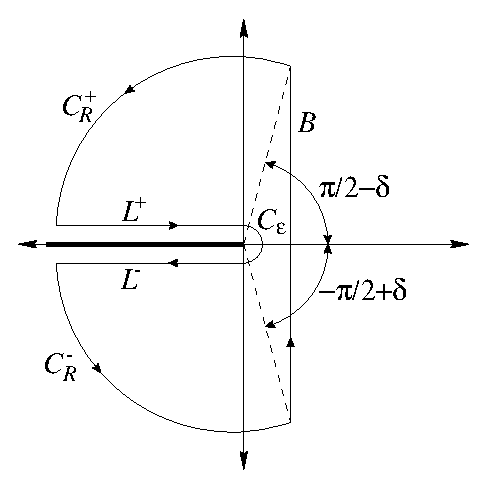
\includegraphics[width=0.4\textwidth]{ode/laplace/sqrts}
    \end{center}
    \caption{Path of integration.}
    \label{one_over_sqrt_s}
  \end{figure}


  Since there are no residues inside the contour, we have
  \[
  \frac{1}{\imath 2 \pi} \left( \int_B + \int_{C_R^+} + \int_{L^+} 
    + \int_{C_\epsilon} + \int_{L^-} + \int_{C_R^-} \right)
  \e^{s t} \frac{1}{\sqrt{s}}\,\dd s = 0.
  \]
  We will evaluate the inverse Laplace transform for $t>0$.


  First we will show that the integral along
  $C_R^+$ vanishes as $R \to \infty$.
  \[
  \int_{C_R^+} \cdots \,\dd s = \int_{\pi/2-\delta}^{\pi/2} \cdots \,\dd \theta + \int_{\pi/2}^\pi \cdots \,\dd \theta.
  \]
  The first integral vanishes by the maximum modulus bound.  Note 
  that the length of the path of integration is less than $2 \alpha$.
  \begin{align*}
    \left| \int_{\pi/2-\delta}^{\pi/2} \cdots \,\dd \theta \right|
    &\leq \left( \max_{s \in C_R^+} 
      \left| \e^{s t} \frac{1}{\sqrt{s}} \right| \right) (2 \alpha) \\
    &= \e^{\alpha t} \frac{1}{\sqrt{R}} (2 \alpha) \\
    &\to 0\ \mathrm{as}\ R \to \infty
  \end{align*}
  The second integral vanishes by Jordan's Lemma.
  A parameterization of $C_R^+$ is $s = R \e^{\imath \theta}$.
  \begin{align*}
    \left| \int_{\pi/2}^{\pi} \e^{R \e^{\imath \theta} t} \frac{1}{\sqrt{R \e^{\imath \theta}}} \,\dd \theta \right|
    &\leq \int_{\pi/2}^{\pi} \left| \e^{R \e^{\imath \theta} t} \frac{1}{\sqrt{R \e^{\imath \theta}}} \right| \,\dd \theta \\
    &\leq \frac{1}{\sqrt{R}} \int_{\pi/2}^{\pi} \e^{R \cos(\theta) t} \,\dd \theta \\
    &\leq \frac{1}{\sqrt{R}} \int_0^{\pi/2} \e^{- R t \sin(\phi)} \,\dd \phi \\
    &< \frac{1}{\sqrt{R}} \frac{\pi}{2 R t} \\
    &\to 0\ \mathrm{as}\ R \to \infty
  \end{align*}
  We could show that the integral along $C_R^-$ vanishes by the same method.
  Now we have
  \[
  \frac{1}{\imath 2 \pi} \left( \int_B + \int_{L^+} + \int_{C_\epsilon} + \int_{L^-} \right)
  \e^{s t} \frac{1}{\sqrt{s}}\,\dd s = 0.
  \]



  We can show that the integral along $C_\epsilon$ vanishes as 
  $\epsilon \to 0$ with the maximum modulus bound.  
  \begin{align*} 
    \left| \int_{C_\epsilon} \e^{s t} \frac{1}{\sqrt{s}} \,\dd s \right|
    &\leq \left(\max_{s \in C_\epsilon} \left| \e^{s t} \frac{1}{\sqrt{s}} 
      \right| \right) (\pi \epsilon) \\
    &< \e^{\epsilon t} \frac{1}{\sqrt{\epsilon}} \pi \epsilon \\
    &\to 0 \quad \mathrm{as}\ \epsilon \to 0
  \end{align*}



  Now we can express the inverse Laplace transform in terms of the integrals
  along $L^+$ and $L^-$.
  \[
  f(t) \equiv \frac{1}{\imath 2 \pi} \int_{\alpha - \imath \infty}^{\alpha + \imath \infty} \e^{s t} \frac{1}{\sqrt{s}}\,\dd s 
  = - \frac{1}{\imath 2 \pi}\int_{L^+} \e^{s t} \frac{1}{\sqrt{s}}\,\dd s 
  - \frac{1}{\imath 2 \pi}\int_{L^-} \e^{s t} \frac{1}{\sqrt{s}}\,\dd s
  \]
  On $L^+$, $s = r \e^{\imath \pi}$, $\dd s = \e^{\imath \pi} \dd r = - \dd r$; 
  on $L^-$, $s = r \e^{-\imath \pi}$, $\dd s = \e^{-\imath \pi} \dd r = - \dd r$.
  We can combine the integrals along the top and bottom of the branch cut.
  \begin{align*}
    f(t)
    &= - \frac{1}{\imath 2 \pi}\int_{\infty}^0 \e^{-r t} \frac{-\imath}{\sqrt{r}} (-1)\,\dd r
    - \frac{1}{\imath 2 \pi} \int_{0}^{\infty} \e^{-r t} \frac{\imath}{\sqrt{r}} (-1)\,\dd r \\
    &= \frac{1}{\imath 2 \pi} \int_0^{\infty} \e^{-r t} \frac{\imath 2}{\sqrt{r}}\,\dd r \\
    \intertext{We make the change of variables $x = r t$.}
    &= \frac{1}{\pi \sqrt{t}} \int_0^\infty \e^{-x} \frac{1}{\sqrt{x}}\,\dd x \\
    \intertext{We recognize this integral as $\Gamma(1/2)$.}
    &= \frac{1}{\pi \sqrt{t}} \Gamma(1/2) \\
    &= \frac{1}{\sqrt{\pi t}}
  \end{align*}

  Thus the inverse Laplace transform of $\frac{1}{\sqrt{s}}$ is
  \[ 
  \boxed{ 
    f(t) = \frac{1}{\sqrt{\pi t}}, \quad \mathrm{for}\ t > 0.
    } 
  \]
\end{Example}







%%------------------------------------------------------------------------------
\subsection{Asymptotic Behavior of $\hat{f}(s)$}



Consider the behavior of
\[
\hat{f}(s) = \int_0^\infty \e^{-s t} f(t) \,\dd t
\]
as $s \to + \infty$.  Assume that $f(t)$ is analytic in a neighborhood
of $t = 0$. Only the behavior of the integrand near $t = 0$ will
make a significant contribution to the value of the integral.  As you
move away from $t = 0$, the $\e^{-s t}$ term dominates.  Thus we could
approximate the value of $\hat{f}(s)$ by replacing $f(t)$ with the first few
terms in its Taylor series expansion about the origin.
\[
\hat{f}(s) \sim \int_0^\infty \e^{-s t} \left[ f(0) + t f'(0) + \frac{t^2}{2} f''(0)
  + \cdots \right] \,\dd t \quad \mathrm{as}\ s \to +\infty
\]
Using
\[
\mathcal{L}\left[ t^n \right] = \frac{n!}{s^{n+1}}
\]
we obtain
\[
\boxed{
  \hat{f}(s) \sim \frac{f(0)}{s} + \frac{f'(0)}{s^2} + \frac{f''(0)}{s^3} +
  \cdots \quad \mathrm{as}\ s \to +\infty.
  }
\]




\begin{Example}
  The Taylor series expansion of $\sin t$ about the origin is
  \[
  \sin t = t - \frac{t^3}{6} + \mathcal{O}(t^5).
  \]
  Thus the Laplace transform of $\sin t$ has the behavior
  \[
  \mathcal{L}[\sin t] \sim \frac{1}{s^2} - \frac{1}{s^4} + \mathcal{O}(s^{-6})
  \quad \mathrm{as}\ s \to + \infty.
  \]
  We corroborate this by expanding $\mathcal{L}[\sin t]$.
  \begin{align*}
    \mathcal{L}[\sin t]
    &= \frac{1}{s^2 + 1} \\
    &= \frac{s^{-2}}{1 + s^{-2}} \\
    &= s^{-2} \sum_{n = 0}^\infty (-1)^n s^{-2n} \\
    &= \frac{1}{s^2} - \frac{1}{s^4} + \mathcal{O}(s^{-6})
  \end{align*}
\end{Example}










%%=============================================================================
\section{Properties of the Laplace Transform}




In this section we will list several useful properties of the Laplace 
transform.  If a result is not derived, it is shown in the Problems section.
Unless otherwise stated, assume that $f(t)$ and $g(t)$ are piecewise
continuous and of exponential order $\alpha$.
\begin{itemize}
\item 
  $\mathcal{L}[a f(t) + b g(t)] = a \mathcal{L}[f(t)] + b \mathcal{L}[g(t)]$
\item 
  $\mathcal{L}[\e^{c t} f(t)] = \hat{f}(s-c)\ \mathrm{for}\ s > c + \alpha$
\item 
  $\mathcal{L}[t^n f(t)] = (-1)^n \frac{d^n}{d s^n}[\hat{f}(s)] 
  \quad \mathrm{for}\ n = 1, 2, \ldots$
\item 
  If $\int_0^\beta \frac{f(t)}{t}\,\dd t$ exists for positive $\beta$ then
  \[ 
  \mathcal{L}\left[ \frac{f(t)}{t} \right] = \int_s^\infty \hat{f}(\sigma)\,\dd \sigma.
  \]
\item 
  $\mathcal{L}\left[ \int_0^t f(\tau)\,\dd \tau \right] = \frac{\hat{f}(s)}{s}$
\item 
  \index{Laplace transforms!of derivatives}
  $\mathcal{L}\left[ \frac{\dd}{\dd t}f(t)\right] = s \hat{f}(s) - f(0)$

  $\mathcal{L}\left[ \frac{\dd^2}{\dd t^2} f(t)\right] = s^2 \hat{f}(s) - s f(0) - f'(0)$

  To derive these formulas,
  \begin{align*}
    \mathcal{L}\left[ \frac{\dd}{\dd t}f(t)\right]
    &= \int_0^\infty \e^{-s t} f'(t)\,\dd t \\
    &= \big[\e^{-s t} f(t) \big]_0^\infty - \int_0^\infty -s \e^{-s t}f(t)\,\dd t \\
    &= -f(0) + s \hat{f}(s)
  \end{align*}
  \begin{align*}
    \mathcal{L}\left[ \frac{\dd^2}{\dd t^2} f(t)\right] 
    &= s \mathcal{L}[f'(t)] - f'(0) \\
    &= s^2 \hat{f}(s) - s f(0) - f'(0)
  \end{align*}

\item Let $f(t)$ and $g(t)$ be continuous.  The convolution of $f(t)$ and 
  \index{convolutions}
  $g(t)$ is defined
  \[
  h(t) = (f*g) = \int_0^t f(\tau)g(t-\tau)\,\dd \tau = \int_0^t f(t-\tau)g(\tau)\,\dd \tau 
  \]
  The \textbf{convolution theorem} states
  \index{convolution theorem!for Laplace transforms}
  \index{Laplace transforms!convolution theorem}
  \[ 
  \hat{h}(s) = \hat{f}(s) \hat{g}(s).
  \]

  To show this,
  \begin{align*}
    \hat{h}(s)    
    &= \int_0^\infty \e^{-s t} \int_0^t f(\tau)g(t-\tau)\,\dd \tau \,\dd t \\
    &= \int_0^\infty \int_\tau^\infty \e^{-s t} f(\tau)g(t-\tau)\,\dd t\,\dd \tau\\
    &= \int_0^\infty \e^{-s \tau}f(\tau) \int_\tau^\infty \e^{-s(t-\tau)} g(t-\tau)\,\dd t\,\dd \tau \\
    &= \int_0^\infty \e^{-s \tau}f(\tau) \,\dd \tau \int_0^\infty \e^{-s \eta}g(\eta)\,\dd \eta \\
    &= \hat{f}(s) \hat{g}(s)
  \end{align*}


\item If $f(t)$ is periodic with period $T$ then
  \[ 
  \mathcal{L}[f(t)] = \frac{\int_0^T \e^{-s t} f(t)\,\dd t}{1-\e^{-s T}}.
  \]
\end{itemize}















\begin{Example}
  Consider the inverse Laplace transform of $\frac{1}{s^3 - s^2}$.
  First we factor the denominator.
  \[ 
  \frac{1}{s^3 - s^2} = \frac{1}{s^2} \frac{1}{s-1} 
  \]
  We know the inverse Laplace transforms of each term.
  \[
  \mathcal{L}^{-1}\left[\frac{1}{s^2}\right] = t, \qquad
  \mathcal{L}^{-1}\left[\frac{1}{s-1}\right] = \e^t
  \]
  We apply the convolution theorem.
  \begin{align*}
    \mathcal{L}^{-1}\left[\frac{1}{s^2} \frac{1}{s-1}\right]
    &= \int_0^t \tau \e^{t-\tau}\,\dd \tau \\
    &= \e^t \left[-\tau \e^{-\tau}\right]_0^t - \e^t \int_0^t -\e^{-\tau}\,\dd \tau\\
    &= -t -1 + \e^t
  \end{align*}
  \[ 
  \boxed{
    \mathcal{L}^{-1}\left[\frac{1}{s^2} \frac{1}{s-1}\right] = \e^t-t-1.
    }
  \]
\end{Example}







\begin{Example}
  We can find the inverse Laplace transform of
  \[ 
  \frac{s^2 + s - 1}{s^3 - 2s^2 + s - 2}
  \]
  with the aid of a table of Laplace transform pairs.
  We factor the denominator.
  \[
  \frac{s^2 + s - 1}{(s - 2)(s - \imath)(s + \imath)}
  \]
  We expand the function in partial fractions and then invert each term.
  \begin{gather*}
    \frac{s^2 + s - 1}{(s - 2)(s - \imath)(s + \imath)} 
    = \frac{1}{s-2} - \frac{\imath / 2}{s - \imath} + \frac{\imath / 2}{s + \imath} 
    \\
    \frac{s^2 + s - 1}{(s - 2)(s - \imath)(s + \imath)} 
    = \frac{1}{s-2} + \frac{1}{s^2 + 1}
    \\
    \boxed{
      \mathcal{L}^{-1}\left[ \frac{1}{s-2} + \frac{1}{s^2+1} \right]
      = \e^{2t} + \sin t
      } 
  \end{gather*}
\end{Example}















%%=============================================================================
\section{Constant Coefficient Differential Equations}









\begin{Example}
  Consider the differential equation
  \[ 
  y' + y = \cos t, \quad \mathrm{for}\ t > 0, \quad y(0) = 1.
  \]
  We take the Laplace transform of this equation.
  \begin{gather*}
    s \hat{y}(s) - y(0) + \hat{y}(s) = \frac{s}{s^2 + 1} \\
    \hat{y}(s) = \frac{s}{(s+1)(s^2+1)} + \frac{1}{s+1} \\
    \hat{y}(s) = \frac{1/2}{s+1} + \frac{1}{2}\frac{s+1}{s^2+1}
  \end{gather*}
  Now we invert $\hat{y}(s)$.
  \[ 
  \boxed{
    y(t) = \frac{1}{2} \e^{-t} + \frac{1}{2} \cos t + \frac{1}{2} \sin t,
    \quad \mathrm{for}\ t > 0
    } 
  \]
  Notice that the initial condition was included when we took the 
  Laplace transform.
\end{Example}







One can see from this example that taking the Laplace transform of a 
constant coefficient differential equation reduces the differential equation
for $y(t)$ to an algebraic equation for $\hat{y}(s)$.






\begin{Example}
  Consider the differential equation
  \[ 
  y'' + y = \cos(2t), \qquad \mathrm{for}\ t>0, \qquad y(0)=1,\ y'(0)=0.
  \]
  We take the Laplace transform of this equation.
  \begin{gather*}
    s^2 \hat{y}(s) - s y(0) - y'(0) + \hat{y}(s) = \frac{s}{s^2+4} \\
    \hat{y}(s) = \frac{s}{(s^2+1)(s^2+4)} + \frac{s}{s^2+1}
  \end{gather*}
  From the table of Laplace transform pairs we know
  \[
  \mathcal{L}^{-1}\left[\frac{s}{s^2+1}\right] = \cos t, \qquad
  \mathcal{L}^{-1}\left[\frac{1}{s^2+4}\right] = \frac{1}{2} \sin(2t).
  \]
  We use the convolution theorem to find the inverse Laplace transform 
  of $\hat{y}(s)$.
  \begin{align*}
    y(t)    
    &= \int_0^t \frac{1}{2}\sin(2\tau) \cos(t-\tau)\,\dd \tau + \cos t \\
    &= \frac{1}{4}\int_0^t \sin(t+\tau) + \sin(3\tau-t)\,\dd \tau + \cos t \\
    &= \frac{1}{4}\left[-\cos(t+\tau) - \frac{1}{3}\cos(3\tau-t)\right]_0^t + \cos t \\
    &= \frac{1}{4}\left(-\cos(2t)+ \cos t -\frac{1}{3}\cos(2t) +
      \frac{1}{3}\cos(t) \right) + \cos t \\
    &= -\frac{1}{3}\cos(2t) + \frac{4}{3} \cos(t) 
  \end{align*}

  Alternatively, we can find the inverse Laplace transform of $\hat{y}(s)$ by
  first finding its partial fraction expansion.
  \begin{align*}
    \hat{y}(s)    
    &= \frac{s/3}{s^2+1} - \frac{s/3}{s^2+4} + \frac{s}{s^2+1} \\
    &= - \frac{s/3}{s^2+4} + \frac{4 s/3}{s^2+1}
  \end{align*}
  \[
  y(t) = - \frac{1}{3} \cos(2 t) + \frac{4}{3} \cos(t)
  \]
\end{Example}









\begin{Example}
  Consider the initial value problem
  \[
  y'' + 5 y' + 2 y = 0, \qquad y(0) = 1, \quad y'(0) = 2.
  \]
  Without taking a Laplace transform, we know that since
  \[
  y(t) = 1 + 2 t + \mathcal{O}(t^2)
  \]
  the Laplace transform has the behavior
  \[
  \hat{y}(s) \sim \frac{1}{s} + \frac{2}{s^2} + \mathcal{O}(s^{-3}),
  \quad \mathrm{as}\ s \to + \infty.
  \]
\end{Example}








%%============================================================================
\section{Systems of Constant Coefficient Differential Equations}




The Laplace transform can be used to transform a system of 
constant coefficient differential equations into a system of 
algebraic equations.  This should not be surprising, as a system of
differential equations can be written as a single differential equation,
and vice versa.





\begin{Example}
  Consider the set of differential equations
  \begin{align*}
    y_1' &= y_2 \\
    y_2' &= y_3 \\
    y_3' &= -y_3 - y_2 - y_1 + t^3 
  \end{align*}
  with the initial conditions
  \[ 
  y_1(0) = y_2(0) = y_3(0) = 0.
  \]

  We take the Laplace transform of this system.
  \begin{align*}
    s \hat{y}_1 - y_1(0) &= \hat{y}_2 \\
    s \hat{y}_2 - y_2(0) &= \hat{y}_3 \\
    s \hat{y}_3 - y_3(0) &= -\hat{y}_3 - \hat{y}_2 - \hat{y}_1 + \frac{6}{s^4}
  \end{align*}
  The first two equations can be written as
  \begin{align*}
    \hat{y}_1 &= \frac{\hat{y}_3}{s^2} \\
    \hat{y}_2 &= \frac{\hat{y}_3}{s}.
  \end{align*}
  We substitute this into the third equation.
  \begin{gather*}
    s \hat{y}_3 = -\hat{y}_3 - \frac{\hat{y}_3}{s} - \frac{\hat{y}_3}{s^2} 
    + \frac{6}{s^4} \\
    (s^3 + s^2 + s + 1)\hat{y}_3 = \frac{6}{s^2} \\
    \hat{y}_3 = \frac{6}{s^2(s^3 + s^2 + s + 1)}.
  \end{gather*}
  We solve for $\hat{y}_1$.
  \begin{gather*}
    \hat{y}_1 = \frac{6}{s^4(s^3 + s^2 + s + 1)} \\
    \hat{y}_1 = \frac{1}{s^4} - \frac{1}{s^3} + \frac{1}{2(s+1)} + \frac{1-s}{2(s^2+1)}
  \end{gather*}
  We then take the inverse Laplace transform of $\hat{y}_1$.
  \[ 
  y_1 = \frac{t^3}{6} - \frac{t^2}{2} + \frac{1}{2} \e^{-t} 
  + \frac{1}{2} \sin t - \frac{1}{2} \cos t.
  \]
  We can find $y_2$ and $y_3$ by differentiating the expression for $y_1$.
  \begin{align*}
    y_2 &= \frac{t^2}{2} - t - \frac{1}{2} \e^{-t}
    + \frac{1}{2} \cos t + \frac{1}{2} \sin t \\
    y_3 &= t - 1 + \frac{1}{2} \e^{-t} - \frac{1}{2} \sin t + \frac{1}{2}\cos t
  \end{align*}
\end{Example}































\raggedbottom
%%=============================================================================
\exercises{
\pagebreak
\flushbottom
\section{Exercises}





%% &(\mathrm{a})\quad f(t) = \cos \omega t \\
\begin{Exercise}
  \label{exercise f(t) = cos omega t}
  Find the Laplace transform of the following functions:
  \begin{enumerate}
  \item $\displaystyle f(t) = \e^{a t}$
  \item $\displaystyle f(t) = \sin(a t)$
  \item $\displaystyle f(t) = \cos(a t)$
  \item $\displaystyle f(t) = \sinh(a t)$
  \item $\displaystyle f(t) = \cosh(a t)$
  \item $\displaystyle f(t) = \frac{ \sin(a t) }{ t }$
  \item $\displaystyle f(t) = \int_0^t \frac{ \sin(a u) }{ u } \,\dd u$
  \item $\displaystyle f(t) = \begin{cases}
      1, &0 \leq t < \pi \\
      0, &\pi \leq t < 2 \pi
    \end{cases}$ \\
    and $f(t+2\pi) = f(t)$ for $t > 0$.  That is, $f(t)$ is periodic for $t > 0$.
  \end{enumerate}

  \hintsolution{f(t) = cos omega t}
\end{Exercise}







%%111111111111111111111111111111111111111111111111111111111111111111111
\begin{Exercise} 
  \label{exercise L(a f + b g) = a L(f) + b L(g)}
  Show that $\mathcal{L}[a f(t) + b g(t)] = a\mathcal{L}[f(t)] 
  + b\mathcal{L}[g(t)]$.

  \hintsolution{L(a f + b g) = a L(f) + b L(g)}
\end{Exercise}


%%222222222222222222222222222222222222222222222222222222222222222222222
\begin{Exercise} %% Shifting property
  \label{exercise L(e c t f) = F(s-c)}
  Show that if $f(t)$ is of exponential order $\alpha$,
  \[ 
  \mathcal{L}[\e^{c t} f(t)] = \hat{f}(s-c)\ \mathrm{for}\ s > c + \alpha.
  \]

  \hintsolution{L(e c t f) = F(s-c)}
\end{Exercise}


%%33333333333333333333333333333333333333333333333333333333333333333333
\begin{Exercise} 
  \label{exercise L(t n f) = }
  Show that
  \[ 
  \mathcal{L}[t^n f(t)] = (-1)^n \frac{d^n}{d s^n}[\hat{f}(s)] 
  \quad \mathrm{for}\ n = 1, 2, \ldots 
  \]

  \hintsolution{L(t n f) = }
\end{Exercise}



%%4444444444444444444444444444444444444444444444444444444444444444444
\begin{Exercise}
  \label{exercise L(f(t)/t)}
  Show that if $\int_0^\beta \frac{f(t)}{t}\,\dd t$ exists for positive $\beta$ then
  \[ 
  \mathcal{L}\left[ \frac{f(t)}{t} \right] 
  = \int_s^\infty \hat{f}(\sigma)\,\dd \sigma.
  \]

  \hintsolution{L(f(t)/t)}
\end{Exercise}






%%555555555555555555555555555555555555555555555555555555555555555555555
\begin{Exercise}
  \label{exercise L(int f(t))}
  Show that
  \[ 
  \mathcal{L}\left[ \int_0^t f(\tau)\,\dd \tau\right] = \frac{\hat{f}(s)}{s}. 
  \]

  \hintsolution{L(int f(t))}
\end{Exercise}








%%666666666666666666666666666666666666666666666666666666666666666666666
\begin{Exercise}
  \label{exercise L(f) f periodic}
  Show that if $f(t)$ is periodic with period $T$ then
  \[ 
  \mathcal{L}[f(t)] = \frac{\int_0^T \e^{-s t} f(t)\,\dd t}{1-\e^{-s T}}.
  \]

  \hintsolution{L(f) f periodic}
\end{Exercise}




%% The function $f(t)$ $t \geq 0$, is periodic with period $2 T$; i.e.
\begin{Exercise}
  \label{exercise L(f) f odd periodic}
  The function $f(t)$ $t \geq 0$, is periodic with period $2 T$; i.e.
  $f(t + 2 T) \equiv f(t)$, and is also odd with period $T$; i.e.
  $f(t + T) = -f(t)$.  Further,
  \[
  \int_0^T f(t) \e^{-s t} \,\dd t = \hat{g}(s).
  \]
  Show that the Laplace transform of $f(t)$ is 
  $\hat{f}(s) = \hat{g}(s) / (1 + \e^{-s T})$.
  Find $f(t)$ such that $\hat{f}(s) = s^{-1} \tanh(s T / 2)$.

  \hintsolution{L(f) f odd periodic}
\end{Exercise}






%%777777777777777777777777777777777777777777777777777777777777777777777777777777
\begin{Exercise}
  \label{exercise L(t nu)}
  Find the Laplace transform of $t^\nu$, $\nu > -1$ by two methods.  
  \begin{enumerate}
  \item 
    Assume that $s$ is complex-valued.  Make the change of variables 
    $z = s t$ and use integration in the complex plane.  
  \item 
    Show that the Laplace transform of $t^\nu$ is an analytic function for
    $\Re(s)>0$.
    Assume that $s$ is real-valued.  Make the change of variables
    $x = s t$ and evaluate the integral.  Then use analytic continuation to 
    extend the result to complex-valued $s$.
  \end{enumerate}

  \hintsolution{L(t nu)}
\end{Exercise}





%% Show that the Laplace transform of $f(t) = \Log t$ is
\begin{Exercise}[mathematica/ode/laplace/laplace.nb]
  \label{exercise L(ln t)}
  Show that the Laplace transform of $f(t) = \ln t$ is
  \[
  \hat{f}(s) = - \frac{\Log s}{s} - \frac{\gamma}{s}, \quad \mathrm{where} \quad
  \gamma = - \int_0^\infty \e^{-t} \ln t \,\dd t.
  \]
  [ $\gamma = 0.5772\ldots$ is known as Euler's constant.]
  
  \hintsolution{L(ln t)}
\end{Exercise}






%%88888888888888888888888888888888888888888888888888888888888888888888888888888
\begin{Exercise}
  \label{exercise L(t nu ln t)}
  Find the Laplace transform of $t^\nu \ln t$.  Write the answer in terms 
  of the digamma function, $\psi(\nu) = \Gamma'(\nu)/\Gamma(\nu)$.
  What is the answer for $\nu = 0$?

  \hintsolution{L(t nu ln t)}
\end{Exercise}







%%888888888888888888888888888888888888888888888888888888888888888888888888888888
\begin{Exercise}
  \label{exercise L(1/(s3-2s2+s-2))}
  Find the inverse Laplace transform of
  \[ 
  \hat{f}(s) = \frac{1}{s^3 - 2s^2 + s - 2} 
  \]
  with the following methods.
  \begin{enumerate}
  \item Expand $\hat{f}(s)$ using partial fractions and then use the table of 
    Laplace transforms.
  \item  Factor the denominator into $(s-2)(s^2+1)$ and then use the 
    convolution theorem.
  \item Use Result \ref{Res_lt_poles}.
  \end{enumerate}

  \hintsolution{L(1/(s3-2s2+s-2))}
\end{Exercise}






%%999999999999999999999999999999999999999999999999999999999999999999999999999999
\begin{Exercise}
  \label{exercise y''+ey'+y=sin t}
  Solve the differential equation
  \[ 
  y'' + \epsilon y' + y = \sin t, \qquad y(0) = y'(0) = 0, \qquad 0 < \epsilon \ll 1 
  \]
  using the Laplace transform.
  This equation represents a weakly damped, driven, linear oscillator.

  \hintsolution{y''+ey'+y=sin t}
\end{Exercise}





%% y'' - t y' + y = 0, \quad y(0) = 0,\ y'(0) = 1,
\begin{Exercise}
  \label{exercise y''-ty'+y=0}
  Solve the problem,
  \[
  y'' - t y' + y = 0, \quad y(0) = 0,\ y'(0) = 1,
  \]
  with the Laplace transform.

  \hintsolution{y''-ty'+y=0}
\end{Exercise}







%%1010101010101010101010101010101010101010101010101010101010101010101010101010
\begin{Exercise}
  \label{exercise relation Laplace Fourier}
  Prove the following relation between the inverse Laplace transform and
  the inverse Fourier transform,
  \[
  \mathcal{L}^{-1} [\hat{f}(s)] = \frac{1}{2\pi} \e^{c t} \mathcal{F}^{-1}
  [\hat{f}(c + \imath \omega)],
  \]
  where $c$ is to the right of the singularities of $\hat{f}(s)$.

  \hintsolution{relation Laplace Fourier}
\end{Exercise}





%% \hat{f}(s) = \left( \frac{\pi}{s} \right)^{1/2} \e^{-2 (a s)^{1/2} }
\begin{Exercise}[mathematica/ode/laplace/laplace.nb]
  \label{exercise F(s)=(pi/s)1/2 e -2(as)1/2}
  Show by evaluating the Laplace inversion integral that if
  \[
  \hat{f}(s) = \left( \frac{\pi}{s} \right)^{1/2} \e^{-2 (a s)^{1/2} }, \quad
  s^{1/2} = \sqrt{s}\ \mathrm{for}\ s > 0,
  \]
  then $f(t) = \e^{-a / t} / \sqrt{t}$.  Hint:  cut the $s$-plane along the 
  negative real axis and deform the contour onto the cut.  Remember that 
  $\int_0^\infty \e^{-a x^2} \cos (b x) \,\dd x = \sqrt{ \pi / 4 a } \e^{-b^2 / 4 a}$.

  \hintsolution{F(s)=(pi/s)1/2 e -2(as)1/2}
\end{Exercise}






%% \frac{d^4 y}{d t^4} - y = t
\begin{Exercise}[mathematica/ode/laplace/laplace.nb]
  \label{exercise y''''-y=t}
  Use Laplace transforms to solve the initial value problem
  \[
  \frac{\dd^4 y}{\dd t^4} - y = t, \qquad
  y(0) = y'(0) = y''(0) = y'''(0) = 0.
  \]

  \hintsolution{y''''-y=t}
\end{Exercise}








%% \frac{\dd y}{\dd t} = \sin t + \int_0^t y(\tau) \cos(t - \tau) \,\dd \tau
\begin{Exercise}[mathematica/ode/laplace/laplace.nb]
  \label{exercise y'=sin t int y cos}
  Solve, by Laplace transforms,
  \[
  \frac{\dd y}{\dd t} = \sin t + \int_0^t y(\tau) \cos(t - \tau) \,\dd \tau, \quad y(0) = 0.
  \]

  \hintsolution{y'=sin t int y cos}
\end{Exercise}







%% \frac{\dd u}{\dd t} + u(t) - u(t-1) = 0, \quad t \geq 0
\begin{Exercise}[mathematica/ode/laplace/laplace.nb]
  \label{exercise u'+u-u(t-1)=0}
  Suppose $u(t)$ satisfies the difference-differential equation
  \[
  \frac{\dd u}{\dd t} + u(t) - u(t-1) = 0, \quad t \geq 0,
  \]
  and the `initial condition' $u(t) = u_0(t)$, $-1 \leq t \leq 0$, where
  $u_0(t)$ is given.  Show that the Laplace transform $\hat{u}(s)$ of $u(t)$
  satisfies
  \[
  \hat{u}(s) = \frac{ u_0(0) }{ 1 + s - \e^{-s} }
  + \frac{ \e^{-s} }{ 1 + s - \e^{-s} } \int_{-1}^0 \e^{-s t} u_0(t) \,\dd t.
  \]
  Find $u(t)$, $t \geq 0$, when $u_0(t) = 1$.  Check the result.

  \hintsolution{u'+u-u(t-1)=0}
\end{Exercise}





%% \frac{\dd^2 y}{\dd t^2} - y = f(t); \qquad y(0) = 1, \quad \frac{\dd y}{\dd t}(0) = 0.
\begin{Exercise}
  \label{exercise f(t)=1,0<t<pi}
  Let the function $f(t)$ be defined by
  \[
  f(t) = 
  \begin{cases}
    1 &0 \leq t < \pi \\
    0 &\pi \leq t < 2 \pi,
  \end{cases}
  \]
  and for all positive values of $t$ so that $f(t+2\pi) = f(t)$.  That is,
  $f(t)$ is periodic with period $2 \pi$.  Find the solution of the intial
  value problem
  \[
  \frac{\dd^2 y}{\dd t^2} - y = f(t); \qquad y(0) = 1, \quad y'(0) = 0.
  \]
  Examine the continuity of the solution at $t = n \pi$, where $n$ is a 
  positive integer, and verify that the solution is continuous and has a 
  continuous derivative at these points.

  \hintsolution{f(t)=1,0<t<pi}
\end{Exercise}









\begin{Exercise}
  \label{exercise y' + int y = e-t}
  Use Laplace transforms to solve
  \[
  \frac{\dd y}{\dd t} + \int_0^t y(\tau) \,\dd \tau = \e^{-t},\quad y(0) = 1.
  \]

  \hintsolution{y' + int y = e-t}
\end{Exercise}





\begin{Exercise}
  \label{exercise circuit i1 i2 q}
  An electric circuit gives rise to the system
  \begin{gather*}
    L \frac{\dd i_1}{\dd t} + R i_1 + q / C = E_0\\
    L \frac{\dd i_2}{\dd t} + R i_2 - q / C = 0\\
    \frac{\dd q}{\dd t} = i_1 - i_2
  \end{gather*}
  with initial conditions
  \[
  i_1(0)=i_2(0)=\frac{E_0}{2R},\quad q(0) = 0.
  \]
  Solve the system by Laplace transform methods and show that
  \[
  i_1= \frac{E_0}{2R}+\frac{E_0}{2 \omega L} \e^{-\alpha t} \sin(\omega t)
  \]
  where
  \[
  \alpha = \frac{R}{2L}\quad \mathrm{and} \quad \omega^2 = \frac{2}{LC} - \alpha^2.
  \]

  \hintsolution{circuit i1 i2 q}
\end{Exercise}






\begin{Exercise}
  \label{exercise y4y4y=4e-t}
  Solve the initial value problem,
  \[
  y''+ 4 y' + 4 y = 4 \e^{-t}, \quad y(0) = 2,~ y'(0) = -3.
  \]

  \hintsolution{y4y4y=4e-t}
\end{Exercise}

















\raggedbottom
}
%%=============================================================================
\hints{
\pagebreak
\flushbottom
\section{Hints}






%% &(\mathrm{a})\quad f(t) = \cos \omega t \\
\begin{Hint}
  \label{hint f(t) = cos omega t}
  Use the differentiation and integration properties of the
  Laplace transform where appropriate.
\end{Hint}






%%11111111111111111111111111111111111111111111111111111111111111111111111111
\begin{Hint}
  \label{hint L(a f + b g) = a L(f) + b L(g)}
  %% CONTINUE
\end{Hint}




%%222222222222222222222222222222222222222222222222222222222222222222222222222222
\begin{Hint}
  \label{hint L(e c t f) = F(s-c)}
  %% CONTINUE
\end{Hint}




%%333333333333333333333333333333333333333333333333333333333333333333333333333333
\begin{Hint}
  \label{hint L(t n f) = }
  If the integral is uniformly convergent and $\frac{\partial g}{\partial s}$ is 
  continuous then
  \[
  \frac{\dd}{\dd s} \int_a^b g(s,t) \,\dd t = \int_a^b \frac{\partial}{\partial s} g(s,t)\,\dd t
  \]
\end{Hint}


%%444444444444444444444444444444444444444444444444444444444444444444444444444444
\begin{Hint}
  \label{hint L(f(t)/t)}
  \[
  \int_s^\infty \e^{-t x}\,\dd t = \frac{1}{x} \e^{-s x}
  \]
\end{Hint}



%%555555555555555555555555555555555555555555555555555555555555555555555555555555
\begin{Hint}
  \label{hint L(int f(t))}
  Use integration by parts.
\end{Hint}


%%666666666666666666666666666666666666666666666666666666666666666666666666666666
\begin{Hint}
  \label{hint L(f) f periodic}
  \[
  \int_0^\infty \e^{-s t} f(t) \,\dd t = \int_{n=0}^\infty 
  \sum_{n T}^{(n+1)T} \e^{-s t} f(t) \,\dd t
  \]
  The sum can be put in the form of a geometric series.
  \[
  \sum_{n = 0}^\infty \alpha^n = \frac{1}{1-\alpha}, \quad \mathrm{for}\ |\alpha| < 1
  \]
\end{Hint}




%% The function $f(t)$ $t \geq 0$, is periodic with period $2 T$; i.e.
\begin{Hint}
  \label{hint L(f) f odd periodic}
  %% CONTINUE
\end{Hint}






%%777777777777777777777777777777777777777777777777777777777777777777777777777777
\begin{Hint}
  \label{hint L(t nu)}
  Write the answer in terms of the Gamma function.
\end{Hint}




%% Show that the Laplace transform of $f(t) = \Log t$ is
\begin{Hint}
  \label{hint L(ln t)}
  %% CONTINUE
\end{Hint}





%%888888888888888888888888888888888888888888888888888888888888888888888888888888
\begin{Hint}
  \label{hint L(t nu ln t)}
  %% CONTINUE
\end{Hint}






%%888888888888888888888888888888888888888888888888888888888888888888888888888888
\begin{Hint}
  \label{hint L(1/(s3-2s2+s-2))}
  %% CONTINUE
\end{Hint}





%%999999999999999999999999999999999999999999999999999999999999999999999999999999
\begin{Hint}
  \label{hint y''+ey'+y=sin t}
  %% CONTINUE
\end{Hint}





%% y'' - t y' + y = 0, \quad y(0) = 0,\ y'(0) = 1,
\begin{Hint}
  \label{hint y''-ty'+y=0}
  %% CONTINUE
\end{Hint}





%%1010101010101010101010101010101010101010101010101010101010101010101010101010
\begin{Hint}
  \label{hint relation Laplace Fourier}
  %% CONTINUE
\end{Hint}








%% \hat{f}(s) = \left( \frac{\pi}{s} \right)^{1/2} \e^{-2 (a s)^{1/2} }
\begin{Hint}
  \label{hint F(s)=(pi/s)1/2 e -2(as)1/2}
  %% CONTINUE
\end{Hint}








%% \frac{d^4 y}{d t^4} - y = t
\begin{Hint}
  \label{hint y''''-y=t}
  %% CONTINUE
\end{Hint}







%% \frac{\dd y}{\dd t} = \sin t + \int_0^t y(\tau) \cos(t - \tau) \,\dd \tau
\begin{Hint}
  \label{hint y'=sin t int y cos}
  %% CONTINUE
\end{Hint}







%% \frac{\dd u}{\dd t} + u(t) - u(t-1) = 0, \quad t \geq 0
\begin{Hint}
  \label{hint u'+u-u(t-1)=0}
  %% CONTINUE
\end{Hint}





%% \frac{\dd^2 y}{\dd t^2} - y = f(t); \qquad y(0) = 1, \quad \frac{\dd y}{\dd t}(0) = 0.
\begin{Hint}
  \label{hint f(t)=1,0<t<pi}
  %% CONTINUE
\end{Hint}






\begin{Hint}
  \label{hint y' + int y = e-t}
  %% CONTINUE
\end{Hint}





\begin{Hint}
  \label{hint circuit i1 i2 q}
  %% CONTINUE
\end{Hint}







\begin{Hint}
  \label{hint y4y4y=4e-t}
  %% CONTINUE
\end{Hint}









\raggedbottom
}
%%=============================================================================
\solutions{
\pagebreak
\flushbottom
\section{Solutions}





%% &(\mathrm{a})\quad f(t) = \cos \omega t \\
\begin{Solution}
  \label{solution f(t) = cos omega t}
  \begin{enumerate}
    %%
    %%
  \item
    \begin{align*}
      \mathcal{L} \left[ \e^{a t} \right]
      &= \int_0^\infty \e^{-s t} \e^{a t} \,\dd t 
      \\
      &= \int_0^\infty \e^{-(s-a) t} \,\dd t 
      \\
      &= \left[ - \frac{\e^{-(s-a) t}}{s-a} \right]_0^\infty
      \quad \mathrm{for}\ \Re(s) > \Re(a)
    \end{align*}
    \[
    \boxed{
      \mathcal{L} \left[ \e^{a t} \right] = \frac{1}{s-a}
      \quad \mathrm{for}\ \Re(s) > \Re(a)
      }
    \]
    %%
    %%
  \item
    \begin{align*}
      \mathcal{L} [ \sin(a t) ]
      &= \int_0^\infty \e^{-s t} \sin(a t) \,\dd t 
      \\
      &= \frac{1}{\imath 2} \int_0^\infty \left( \e^{(-s + \imath a) t} -  \e^{(-s - \imath a) t} \right) \,\dd t 
      \\
      &= \frac{1}{\imath 2} \left[ \frac{ - \e^{(-s + \imath a) t} }{s - \imath a}
        + \frac{ \e^{(-s - \imath a) t} }{ s + \imath a } \right]_0^\infty,
      \quad \mathrm{for}\ \Re(s) > 0
      \\
      &= \frac{1}{\imath 2} \left( \frac{1}{ s - \imath a } - \frac{1}{ s + \imath a } \right) 
    \end{align*}
    \[
    \boxed{
      \mathcal{L} [ \sin(a t) ] = \frac{ a }{ s^2 + a^2 }
      \quad \mathrm{for}\ \Re(s) > 0
      }
    \]
    %%
    %%
  \item
    \begin{align*}
      \mathcal{L} [ \cos(a t) ]
      &= \mathcal{L} \left[ \frac{\dd}{\dd t} \frac{\sin(a t)}{a} \right] 
      \\
      &= s \mathcal{L} \left[ \frac{\sin(a t)}{a} \right] - \sin(0)
    \end{align*}
    \[
    \boxed{
      \mathcal{L} [ \cos(a t) ] = \frac{ s }{ s^2 + a^2 }
      \quad \mathrm{for}\ \Re(s) > 0
      }
    \]
    %%
    %%
  \item
    \begin{align*}
      \mathcal{L} [ \sinh(a t) ]
      &= \int_0^\infty \e^{-s t} \sinh(a t) \,\dd t 
      \\
      &= \frac{1}{2} \int_0^\infty \left( \e^{(-s + a) t} - \e^{(-s - a) t} \right) \,\dd t 
      \\
      &= \frac{1}{2} \left[ \frac{ - \e^{(-s + a) t} }{s - a}
        + \frac{ \e^{(-s - a) t} }{ s + a } \right]_0^\infty
      \quad \mathrm{for}\ \Re(s) > |\Re(a)| 
      \\
      &= \frac{1}{2} \left( \frac{1}{ s - a } 
        - \frac{1}{ s + a } \right) 
    \end{align*}
    \[
    \boxed{
      \mathcal{L} [ \sinh(a t) ] = \frac{ a }{ s^2 - a^2 }
      \quad \mathrm{for}\ \Re(s) > |\Re(a)|
      }
    \]
    %%
    %%
  \item
    \begin{align*}
      \mathcal{L} [ \cosh(a t) ]
      &= \mathcal{L} \left[ \frac{\dd}{\dd t} \frac{\sinh(a t)}{a} \right] 
      \\
      &= s \mathcal{L} \left[ \frac{\sinh(a t)}{a} \right] - \sinh(0)
    \end{align*}
    \[
    \boxed{
      \mathcal{L} [ \cosh(a t) ] = \frac{ s }{ s^2 - a^2 }
      \quad \mathrm{for}\ \Re(s) > |\Re(a)|
      }
    \]
    %%
    %%
  \item
    First note that
    \[
    \mathcal{L} \left[ \frac{\sin(a t)}{t} \right](s)
    = \int_s^\infty \mathcal{L} [ \sin(a t) ](\sigma) \,\dd \sigma.
    \]
    Now we use the Laplace transform of $\sin(a t)$ to compute the Laplace 
    transform of $\sin(a t)/t$.
    \begin{align*}
      \mathcal{L} \left[ \frac{\sin(a t)}{t} \right]
      &= \int_s^\infty \frac{a}{ \sigma^2 + a^2 } \,\dd \sigma \\
      &= \int_s^\infty \frac{1}{ (\sigma/a)^2 + 1 } \,
      \frac{ d \sigma }{ a } \\
      &= \left[ \arctan\left( \frac{\sigma}{a} \right) \right]_s^\infty \\
      &= \frac{\pi}{2} - \arctan \left( \frac{s}{a} \right)
    \end{align*}
    \[
    \boxed{
      \mathcal{L} \left[ \frac{\sin(a t)}{t} \right] 
      = \arctan \left( \frac{ a }{ s } \right)
      }
    \]
    %%
    %%
  \item
    \[
    \mathcal{L} \left[ \int_0^t \frac{ \sin(a \tau) }{ \tau } \,\dd \tau \right]
    = \frac{1}{s} \mathcal{L} \left[ \frac{ \sin(a t) }{ t } \right]
    \]
    \[
    \boxed{
      \mathcal{L} \left[ \int_0^t \frac{ \sin(a \tau) }{ \tau } \,\dd \tau \right]
      = \frac{1}{s} \arctan \left( \frac{ a }{ s } \right)
      }
    \]
    %%
    %%
  \item
    \begin{align*}
      \mathcal{L}[ f(t) ]
      &= \frac{ \int_0^{2\pi} \e^{-s t} f(t) \,\dd t }{ 1 - \e^{-2 \pi s} } \\
      &= \frac{ \int_0^\pi \e^{-s t} \,\dd t }{ 1 - \e^{-2 \pi s} } \\
      &= \frac{ 1 - \e^{- \pi s}}{ s ( 1 - \e^{-2 \pi s} ) } 
    \end{align*}
    \[
    \boxed{
      \mathcal{L}[ f(t) ] = \frac{ 1 }{ s ( 1 + \e^{- \pi s} ) }
      }
    \]
  \end{enumerate}
\end{Solution}







%%1111111111111111111111111111111111111111111111111111111111111111111
\begin{Solution} %% Linearity of Laplace transform.
  \label{solution L(a f + b g) = a L(f) + b L(g)}
  \begin{align*}
    \mathcal{L}[a f(t) + b g(t)] 
    &= \int_0^\infty \e^{-s t} \big(a f(t) + b g(t)\big)\,\dd t \\
    &= a \int_0^\infty \e^{-s t} f(t)\,\dd t 
    + b \int_0^\infty \e^{-s t} g(t)\,\dd t \\
    &= a \mathcal{L}[f(t)] + b \mathcal{L}[g(t)]
  \end{align*}
\end{Solution}








%%2222222222222222222222222222222222222222222222222222222222222222222222
\begin{Solution} %% Shifting property
  \label{solution L(e c t f) = F(s-c)}
  If $f(t)$ is of exponential order $\alpha$, then $\e^{c t} f(t)$ is of 
  exponential order $c + \alpha$.
  \begin{align*}
    \mathcal{L}[\e^{c t} f(t)]
    &= \int_0^\infty \e^{-s t} \e^{c t} f(t)\,\dd t \\
    &= \int_0^\infty \e^{-(s-c) t} f(t)\,\dd t \\
    &= \hat{f}(s-c)\ \mathrm{for}\ s > c + \alpha
  \end{align*}
\end{Solution}




%%333333333333333333333333333333333333333333333333333333333333333333333
\begin{Solution}
  \label{solution L(t n f) = }
  First consider the Laplace transform of $t^0 f(t)$.
  \[
  \mathcal{L}[t^0 f(t)] = \hat{f}(s)
  \]
  Now consider the Laplace transform of $t^n f(t)$ for $n \geq 1$.
  \begin{align*}
    \mathcal{L}[t^n f(t)]
    &= \int_0^\infty \e^{-s t} t^n f(t)\,\dd t \\
    &= -\frac{\dd}{\dd s} \int_0^\infty \e^{-s t} t^{n-1} f(t)\,\dd t \\
    &= -\frac{\dd}{\dd s} \mathcal{L}[t^{n-1} f(t)]
  \end{align*}
  Thus we have a difference equation for the Laplace transform of $t^n f(t)$ 
  with the solution
  \[
  \mathcal{L}[t^n f(t)] = (-1)^n \frac{d^n}{d s^n} \mathcal{L}[t^0 f(t)]\ 
  \mathrm{for}\ n \in \mathbb{Z}^{0+},
  \]
  \[
  \boxed{
    \mathcal{L}[t^n f(t)] = (-1)^n \frac{d^n}{d s^n} \hat{f}(s)\ 
    \mathrm{for}\ n \in \mathbb{Z}^{0+}.
    }
  \]
\end{Solution}





%%44444444444444444444444444444444444444444444444444444444444444444444
\begin{Solution}
  \label{solution L(f(t)/t)}
  If $\int_0^\beta \frac{f(t)}{t}\,\dd t$ exists for positive $\beta$ and 
  $f(t)$ is of exponential order $\alpha$ then the Laplace transform
  of $f(t)/t$ is defined for $s > \alpha$.
  \begin{align*}
    \mathcal{L}\left[\frac{f(t)}{t}\right]
    &= \int_0^\infty \e^{-s t} \frac{1}{t} f(t)\,\dd t \\
    &= \int_0^\infty \int_s^\infty \e^{-\sigma t}\,\dd \sigma  \, f(t)\,\dd t \\
    &= \int_s^\infty \int_0^\infty e^{-\sigma t}f(t)\,\dd t\,\dd \sigma \\
    &= \int_s^\infty \hat{f}(\sigma)\,\dd \sigma
  \end{align*}
\end{Solution}




%%5555555555555555555555555555555555555555555555555555555555555555555
\begin{Solution}
  \label{solution L(int f(t))}
  \begin{align*}
    \mathcal{L}\left[ \int_0^t f(\tau)\,\dd \tau \right]
    &= \int_0^\infty \e^{-s t} \int_0^t f(\tau)\,\dd \tau\,\dd x 
    \\
    &= \left[ -\frac{\e^{-s t}}{s} \int_0^t f(\tau)\,\dd \tau \right]_0^\infty
    - \int_0^\infty -\frac{\e^{-s t}}{s} 
    \frac{\dd}{\dd t} \left[ \int_0^t f(\tau)\,\dd \tau \right]\,\dd t 
    \\
    &= \frac{1}{s} \int_0^\infty \e^{-s t} f(t)\,\dd t 
    \\
    &= \frac{1}{s} \hat{f}(s) 
  \end{align*}
\end{Solution}










%%6666666666666666666666666666666666666666666666666666666666666666666
\begin{Solution}
  \label{solution L(f) f periodic}
  $f(t)$ is periodic with period $T$.
  \begin{align*}
    \mathcal{L}[f(t)]
    &= \int_0^\infty \e^{-s t} f(t)\,\dd t \\
    &= \int_0^T \e^{-s t} f(t)\,\dd t + \int_T^{2T} \e^{-s t} f(t)\,\dd t + \cdots \\
    &= \sum_{n=0}^\infty \int_{n T}^{(n+1)T} \e^{-s t} f(t)\,\dd t \\
    &= \sum_{n=0}^\infty \int_0^T \e^{-s (t+n T)} f(t+n T)\,\dd t \\
    &= \sum_{n=0}^\infty \e^{-s n T} \int_0^T \e^{-s t} f(t)\,\dd t \\
    &= \int_0^T \e^{-s t} f(t)\,\dd t \sum_{n=0}^\infty \e^{-s n T} \\
    &= \frac{\int_0^T \e^{-s t} f(t)\,\dd t}{1-\e^{-s T}}
  \end{align*}
\end{Solution}







%% The function $f(t)$ $t \geq 0$, is periodic with period $2 T$; i.e.
\begin{Solution}
  \label{solution L(f) f odd periodic}
  \begin{align*}
    \hat{f}(s)    
    &= \int_0^\infty \e^{-s t} f(t) \,\dd t \\
    &= \sum_0^n  \int_{n T}^{(n+1) T} \e^{-s t} f(t) \,\dd t \\
    &= \sum_0^n \int_0^T \e^{-s (t + n T)} f(t + n T) \,\dd t \\
    &= \sum_0^n \e^{-s n T} \int_0^T \e^{-s t} (-1)^n f(t) \,\dd t \\
    &= \int_0^T \e^{-s t} f(t) \,\dd t \sum_0^n (-1)^n \left( \e^{-s T} \right)^n 
  \end{align*}
  \[
  \boxed{
    \hat{f}(s) = \frac{ \hat{g}(s) }{ 1 + \e^{-s T} }, \quad \mathrm{for}\ \Re(s) > 0
    }
  \]

  Consider $\hat{f}(s) = s^{-1} \tanh(s T/2)$.
  \begin{align*}
    s^{-1} \tanh(s T / 2)
    &= s^{-1} \frac{ \e^{s T / 2} - \e^{-s T / 2} }{ \e^{s T / 2} + \e^{-s T / 2} } \\
    &= s^{-1} \frac{ 1 - \e^{-s T} }{ 1 + \e^{-s T} } \\
  \end{align*}
  We have
  \[
  \hat{g}(s) \equiv \int_0^T f(t) \e^{-s t} \,\dd t = \frac{ 1 - \e^{-s t} }{s}.
  \]
  By inspection we see that this is satisfied for $f(t) = 1$ for 
  $0 < t < T$.  We conclude:
  \[
  \boxed{
    f(t) = 
    \begin{cases}
      1 &\mathrm{for}\ t \in [2 n T \ldots (2n+1) T), \\
      -1 &\mathrm{for}\ t \in [(2 n+1) T \ldots (2n+2) T),
    \end{cases}
    }
  \]
  where $n \in \mathbb{Z}$.
\end{Solution}







%%777777777777777777777777777777777777777777777777777777777777777777777777777
\begin{Solution}
  \label{solution L(t nu)}
  The Laplace transform of $t^\nu$, $\nu > -1$ is
  \[ 
  \hat{f}(s) = \int_0^\infty \e^{-s t} t^\nu \,\dd t. 
  \]
  Assume $s$ is complex-valued. The integral converges for
  $\Re(s) > 0$ and $\nu > -1$.

  \paragraph{Method 1.}
  We make the change of variables $z = s t$.
  \begin{align*}
    \hat{f}(s)    
    &= \int_C \e^{-z} \left(\frac{z}{s}\right)^\nu \frac{1}{s} \,\dd z \\
    &= s^{-(\nu+1)} \int_C \e^{-z} z^{\nu}\,\dd z
  \end{align*}
  $C$ is the path from $0$ to $\infty$ along $\arg(z) = \arg(s)$.
  (Shown in Figure~\ref{Cpath}).

  \begin{figure}[h!]
    \begin{center}
      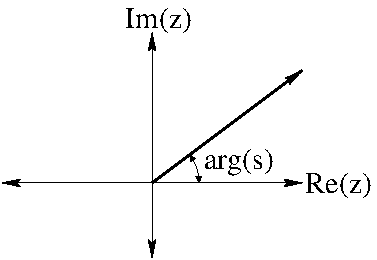
\includegraphics[width=0.25\textwidth]{ode/laplace/cpath}
    \end{center}
    \caption{The path of integration.}
    \label{Cpath}
  \end{figure}



  Since the integrand is analytic in the domain $\epsilon < r < R$, $0 < \theta < \arg(s)$,
  the integral along the boundary of this domain vanishes.
  \[ 
  \left( \int_\epsilon^R + \int_R^{R \e^{\imath \arg(s)}} + \int_{R \e^{\imath \arg(s)}}^{\epsilon \e^{\imath \arg(s)}} 
    + \int_{\epsilon \e^{\imath \arg(s)}}^\epsilon \right) \e^{-z} z^\nu \, \dd z = 0 
  \]
  We show that the integral along $C_R$, the circular arc of radius $R$, 
  vanishes as $R \to \infty$ with the maximum modulus integral bound.
  \begin{align*}
    \left| \int_{C_R} \e^{-z} z^\nu \,\dd z \right|
    &\leq R | \arg(s) | \max_{z \in C_R} \left| \e^{-z} z^\nu \right| \\
    &= R |\arg(s)| \e^{-R \cos(\arg(s))} R^\nu \\
    &\to 0 \quad \mathrm{as}\ R \to \infty.
  \end{align*}
  The integral along $C_\epsilon$, the circular arc of radius $\epsilon$, 
  vanishes as $\epsilon \to 0$.  We demonstrate this with the maximum modulus 
  integral bound.
  \begin{align*}
    \left| \int_{C_\epsilon} \e^{-z} z^\nu \,\dd z \right|
    &\leq \epsilon | \arg(s) | \max_{z \in C_\epsilon} \left| \e^{-z} z^\nu \right| \\
    &= \epsilon |\arg(s)| \e^{-\epsilon \cos(\arg(s))} \epsilon^\nu \\
    &\to 0 \quad \mathrm{as}\ \epsilon \to 0.
  \end{align*}


  Taking the limit as $\epsilon \to 0$ and $R \to \infty$, we see that the integral along $C$
  is equal to the integral along the real axis.
  \[ 
  \int_C \e^{-z} z^\nu \,\dd z = \int_0^\infty \e^{-z} z^\nu \, dz
  \]
  We can evaluate the Laplace transform of $t^\nu$ in terms of this integral.
  \begin{gather*}
    \mathcal{L} \left[ t^\nu \right] = s^{-(\nu+1)} \int_0^\infty \e^{-t} t^{\nu} \,\dd t \\
    \boxed{
      \mathcal{L} \left[ t^\nu \right] = \frac{\Gamma(\nu + 1)}{s^{\nu+1}}
      } 
  \end{gather*}
  In the case that $\nu$ is a non-negative integer $\nu = n > -1$ we can write 
  this in terms of the factorial.
  \[
  \mathcal{L} \left[ t^n \right] = \frac{n!}{s^{n+1}}
  \]



  \paragraph{Method 2.}
  First note that the integral
  \[
  \hat{f}(s) = \int_0^\infty \e^{-s t} t^\nu \,\dd t
  \]
  exists for $\Re(s) > 0$.  It converges uniformly for $\Re(s) \geq c > 0$.
  On this domain of uniform convergence we can interchange differentiation
  and integration.
  \begin{align*}
    \frac{\dd \hat{f}}{\dd s} 
    &= \frac{\dd}{\dd s} \int_0^\infty \e^{-s t} t^\nu \,\dd t \\
    &= \int_0^\infty \frac{\partial}{\partial s} \left( \e^{-s t} t^{\nu} \right) \,\dd t \\
    &= \int_0^\infty -t \e^{-s t} t^{\nu} \,\dd t \\
    &= - \int_0^\infty \e^{-s t} t^{\nu+1} \,\dd t 
  \end{align*}
  Since $\hat{f}'(s)$ is defined for $\Re(s) > 0$, $\hat{f}(s)$ is analytic for 
  $\Re(s)>0$.

  Let $\sigma$ be real and positive.  We make the change of variables $x = \sigma t$.
  \begin{align*}
    \hat{f}(\sigma)    
    &= \int_0^\infty \e^{-x} \left( \frac{x}{\sigma} \right)^\nu \frac{1}{\sigma} \,\dd x \\
    &= \sigma^{-(\nu+1)} \int_0^\infty \e^{-x} x^{\nu} \,\dd x \\
    &= \frac{\Gamma(\nu+1)}{\sigma^{\nu + 1}}
  \end{align*}
  Note that the function
  \[
  \hat{f}(s) = \frac{\Gamma(\nu+1)}{s^{\nu + 1}}
  \]
  is the analytic continuation of $\hat{f}(\sigma)$.
  Thus we can define the Laplace transform for all
  complex $s$ in the right half plane.
  \[ 
  \boxed{ 
    \hat{f}(s) = \frac{\Gamma(\nu+1)}{s^{\nu + 1}}
    } 
  \]
\end{Solution}









%% Show that the Laplace transform of $f(t) = \Log t$ is
\begin{Solution}
  \label{solution L(ln t)}
  Note that $\hat{f}(s)$ is an analytic function for $\Re(s) > 0$.  
  Consider real-valued $s > 0$.  By definition, $\hat{f}(s)$ is 
  \[
  \hat{f}(s) = \int_0^\infty \e^{-s t} \ln t \,\dd t.
  \]
  We make the change of variables $x = s t$.
  \begin{align*}
    \hat{f}(s)
    &= \int_0^\infty \e^{-x} \ln \left( \frac{x}{s} \right) \, \frac{\dd x}{s} \\
    &= \frac{1}{s} \int_0^\infty \e^{-x} \left( \ln x - \ln s \right) \,\dd x \\
    &= - \frac{\ln |s|}{s} \int_0^\infty \e^{-x} \,\dd x 
    + \frac{1}{s} \int_0^\infty \e^{-x} \ln x \,\dd x \\
    &= - \frac{\ln s}{s} - \frac{\gamma}{s}, \quad \mathrm{for real}\ s > 0
  \end{align*}
  The analytic continuation of $\hat{f}(s)$ into the right half-plane is
  \[ 
  \boxed{
    \hat{f}(s) = - \frac{\Log s}{s} - \frac{\gamma}{s}.
    }
  \]
\end{Solution}







%%88888888888888888888888888888888888888888888888888888888888888888888888888888
%% CONTINUE: Check
\begin{Solution}
  \label{solution L(t nu ln t)}
  Define
  \[
  \hat{f}(s) = \mathcal{L}[t^\nu \ln t] = \int_0^\infty \e^{-s t} t^\nu \ln t \,\dd t.
  \]
  This integral defines $\hat{f}(s)$ for $\Re(s) > 0$.  Note that the integral
  converges uniformly for $\Re(s) \geq c > 0$.  On this domain we can
  interchange differentiation and integration.
  \[
  \hat{f}'(s) = \int_0^\infty \frac{\partial}{\partial s} \left( \e^{-s t} t^\nu \ln t \right) \,\dd t
  = - \int_0^\infty t \e^{-s t} t^\nu \Log t \,\dd t
  \]
  Since $\hat{f}'(s)$ also exists for $\Re(s) > 0$, 
  $\hat{f}(s)$ is analytic in that domain.

  Let $\sigma$ be real and positive.  
  We make the change of variables $x = \sigma t$.
  \begin{align*}
    \hat{f}(\sigma) 
    &= \mathcal{L} \left[ t^\nu \ln t \right] \\
    &= \int_0^\infty \e^{-\sigma t} t^\nu \ln t \,\dd t \\
    &= \int_0^\infty \e^{-x} \left( \frac{x}{\sigma} \right)^\nu 
    \ln \frac{x}{\sigma} \frac{1}{\sigma}\,\dd x \\
    &= \frac{1}{\sigma^{\nu+1}} \int_0^\infty \e^{-x} x^\nu ( \ln x - \ln \sigma ) \,\dd x \\
    &= \frac{1}{\sigma^{\nu+1}} \left( \int_0^\infty \e^{-x} x^\nu \ln x \,\dd x
      - \ln \sigma \int_0^\infty \e^{-x} x^\nu \,\dd x \right) \\
    &= \frac{1}{\sigma^{\nu+1}} \left( \int_0^\infty \frac{\partial}{\partial \nu} \left( 
        \e^{-x} x^\nu \right) \,\dd x - \ln \sigma \Gamma(\nu+1) \right) \\
    &= \frac{1}{\sigma^{\nu+1}} \left( \frac{\dd}{\dd \nu} \int_0^\infty 
      \e^{-x} x^\nu \,\dd x - \ln \sigma \Gamma(\nu+1) \right) \\
    &= \frac{1}{\sigma^{\nu+1}} \left( \frac{\dd}{\dd \nu} \Gamma(\nu+1)
      - \ln \sigma \Gamma(\nu+1) \right) \\
    &= \frac{1}{\sigma^{\nu+1}} \Gamma(\nu+1) \left( \frac{\Gamma'(\nu+1)}
      {\Gamma(\nu+1)} - \ln \sigma \right) \\
    &= \frac{1}{\sigma^{\nu+1}} \Gamma(\nu+1) \left( \psi(\nu+1) - \ln \sigma \right) 
  \end{align*}
  Note that the function
  \[
  \hat{f}(s) = \frac{1}{s^{\nu+1}} \Gamma(\nu+1) \left( \psi(\nu+1) - \ln s \right) 
  \]
  is an analytic continuation of $\hat{f}(\sigma)$.  Thus we can define the Laplace
  transform for all $s$ in the right half plane.
  \[
  \boxed{
    \mathcal{L}[t^\nu \ln t] = \frac{1}{s^{\nu+1}} \Gamma(\nu+1) 
    \left( \psi(\nu+1) - \ln s \right) \quad \mathrm{for}\ \Re(s) > 0.
    }
  \]
  For the case $\nu = 0$, we have
  \begin{gather*}
    \mathcal{L}[\ln t] = \frac{1}{s^1} \Gamma(1) \left( \psi(1) - \ln s \right) \\
    \boxed{
      \mathcal{L}[\ln t] = \frac{-\gamma - \ln s}{s},
      }
  \end{gather*}
  where $\gamma$ is Euler's constant
  \[
  \gamma = \int_0^\infty \e^{-x} \ln x \,\dd x = 0.5772156629\ldots
  \]
\end{Solution}







%%888888888888888888888888888888888888888888888888888888888888888888888888888888
\begin{Solution}
  \label{solution L(1/(s3-2s2+s-2))}
  \textbf{Method 1.}
  We factor the denominator.
  \[ 
  \hat{f}(s) = \frac{1}{(s-2)(s^2+1)} = \frac{1}{(s-2)(s-\imath)(s+\imath)}
  \]
  We expand the function in partial fractions and simplify the result.
  \begin{gather*}
    \frac{1}{(s-2)(s-\imath)(s+\imath)} 
    = \frac{1/5}{s-2} 
    - \frac{(1 - \imath 2)/10}{s - \imath}
    - \frac{(1 + \imath 2)/10}{s + \imath} \\
    \hat{f}(s) = \frac{1}{5} \frac{1}{s-2} - \frac{1}{5} \frac{s+2}{s^2+1} 
  \end{gather*}
  We use a table of Laplace transforms to do the inversion.
  \begin{gather*}
    \mathcal{L} [\e^{2t}] = \frac{1}{s-2}, \quad
    \mathcal{L}[\cos t] =  \frac{s}{s^2+1}, \quad
    \mathcal{L}[\sin t] =  \frac{1}{s^2+1} \\
    \boxed{ 
      f(t) = \frac{1}{5} \left( \e^{2t} - \cos t - 2 \sin t \right)
      }
  \end{gather*}

  \textbf{Method 2.}
  We factor the denominator.
  \[ 
  \hat{f}(s) = \frac{1}{s-2} \frac{1}{s^2+1} 
  \]
  From a table of Laplace transforms we note
  \[ 
  \mathcal{L} [\e^{2t} ] = \frac{1}{s-2}, \qquad
  \mathcal{L}[\sin t] = \frac{1}{s^2+1}. 
  \]
  We apply the convolution theorem.
  \begin{gather*}
    f(t) = \int_0^t \sin \tau \ \e^{2(t-\tau)} \,\dd \tau \\
    \boxed{ 
      f(t) = \frac{1}{5} \left( \e^{2t} - \cos t - 2 \sin t \right)
      }
  \end{gather*}

  \paragraph{Method 3.}
  We factor the denominator.
  \[ 
  \hat{f}(s) = \frac{1}{(s-2)(s-\imath)(s+\imath)}
  \]
  $\hat{f}(s)$ is analytic except for poles and vanishes at infinity.
  \begin{align*}
    f(t)    
    &= \sum_{s_n = 2,\imath,-\imath} \Res\left(\frac{\e^{s t}}{(s-2)(s-\imath)(s+\imath)}, 
      s_n \right) \\
    &= \frac{\e^{2t}}{(2-\imath)(2+\imath)} + \frac{\e^{\imath t}}{(\imath-2)(\imath 2)}
    + \frac{\e^{-\imath t}}{(-\imath-2)(-\imath 2)} \\
    &= \frac{\e^{2t}}{5} + \frac{(-1+\imath 2)\e^{\imath t}}{10}
    + \frac{(-1-\imath 2)\e^{-\imath t}}{10} \\
    &= \frac{\e^{2t}}{5} + - \frac{\e^{\imath t} + \e^{-\imath t}}{10}
    + \imath \frac{\e^{\imath t} - \e^{-\imath t}}{5}
  \end{align*}
  \[ 
  \boxed{ 
    f(t) = \frac{1}{5} \left( \e^{2t} - \cos t - 2 \sin t \right)
    } 
  \]
\end{Solution}














%%999999999999999999999999999999999999999999999999999999999999999999999999999999
\begin{Solution}
  \label{solution y''+ey'+y=sin t}
  \[ 
  y'' + \epsilon y' + y = \sin t, \qquad y(0) = y'(0) = 0, \qquad 0 < \epsilon \ll 1
  \]
  We take the Laplace transform of this equation.
  \begin{gather*}
    (s^2 \hat{y}(s) - s y(0) - y'(0)) + \epsilon (s \hat{y}(s) - y(0)) + \hat{y}(s)
    = \mathcal{L}[ \sin(t) ] \\
    (s^2 + \epsilon s + 1)\hat{y}(s) = \mathcal{L}[ \sin(t) ] \\
    \hat{y}(s) = \frac{1}{s^2 + \epsilon s + 1} \mathcal{L}[ \sin(t) ] \\
    \hat{y}(s) = \frac{1}{ (s+ \frac{\epsilon}{2})^2 + 1 - \frac{\epsilon^2}{4} } 
    \mathcal{L}[ \sin(t) ]
  \end{gather*}
  We use a table of Laplace transforms to find the inverse Laplace transform
  of the first term.
  \[
  \mathcal{L}^{-1} \left[ \frac{1}{(s+ \frac{\epsilon}{2})^2 + 1 - \frac{\epsilon^2}{4}} \right]
  = \frac{1}{\sqrt{1 - \frac{\epsilon^2}{4}}} \e^{-\epsilon t / 2}
  \sin \left( \sqrt{1 - \frac{\epsilon^2}{4}} t \right)
  \]
  We define
  \[
  \alpha = \sqrt{1 - \frac{\epsilon^2}{4}}
  \]
  to get rid of some clutter.  Now we apply the convolution theorem to invert
  \footnote{Evaluate the convolution integral by inspection.}
  $\hat{y}{s}$.
  \begin{gather*}
    y(t) = \int_0^t \frac{1}{\alpha} \e^{-\epsilon \tau / 2} \sin \left( \alpha \tau \right) \sin (t - \tau) \,\dd \tau \\
    \boxed{
      y(t) =  \e^{-\epsilon t/2} \left( \frac{1}{\epsilon} \cos \left( \alpha t
        \right) + \frac{1}{2 \alpha} \sin \left( \alpha t
        \right) \right) - \frac{1}{\epsilon} \cos t
      }
  \end{gather*}
  The solution is plotted in Figure~\ref{damped_driven} for $\epsilon = 0.05$.

  \begin{figure}[h!]
    \begin{center}
      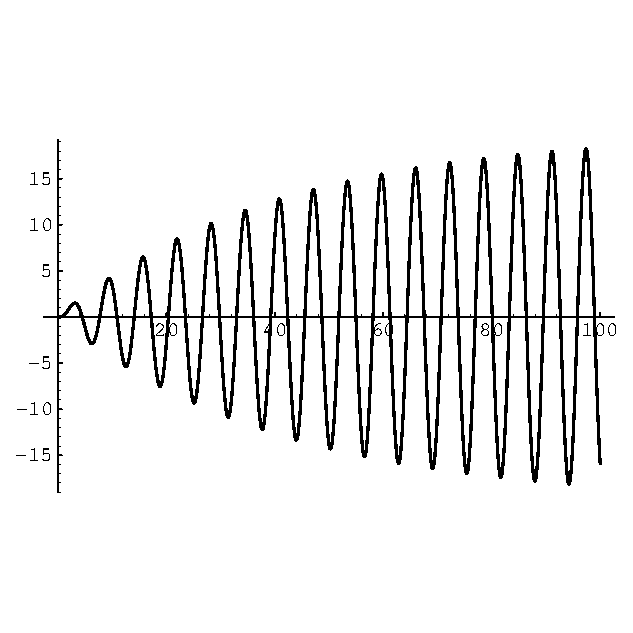
\includegraphics[width=0.6\textwidth]{ode/laplace/dampdriv}
    \end{center}
    \caption{The weakly damped, driven oscillator.}
    \label{damped_driven}
  \end{figure}

\end{Solution}















%% y'' - t y' + y = 0, \quad y(0) = 0,\ y'(0) = 1,
\begin{Solution}
  \label{solution y''-ty'+y=0}
  We consider the solutions of
  \[
  y'' - t y' + y = 0, \quad y(0) = 0,\ y'(0) = 1
  \]
  which are of exponential order $\alpha$ for any $\alpha > 0$.
  We take the Laplace transform of the differential equation.
  \begin{gather*}
    s^2 \hat{y} - 1 + \frac{\dd}{\dd s} \left( s \hat{y} \right) + \hat{y} = 0 \\
    \hat{y}' + \left( s + \frac{2}{s} \right) \hat{y} = \frac{1}{s} \\
    \hat{y}(s) = \frac{1}{s^2} + c \frac{\e^{-s^2/2}}{s^2}
  \end{gather*}
  We use that
  \[
  \hat{y}(s) \sim \frac{y(0)}{s} + \frac{y'(0)}{s^2} + \cdots
  \]
  to conclude that $c = 0$.
  \begin{gather*}
    \hat{y}(s) = \frac{1}{s^2} \\
    \boxed{
      y(t) = t
      }
  \end{gather*}
\end{Solution}










%%1010101010101010101010101010101010101010101010101010101010101010101010101010
\begin{Solution}
  \label{solution relation Laplace Fourier}
  \[
  \mathcal{L}^{-1}[\hat{f}(s)] = \frac{1}{\imath 2 \pi} \int_{c - \imath \infty}^{c + \imath \infty}
  \e^{s t} \hat{f}(s) \,\dd s
  \]
  First we make the change of variable $s = c + \sigma$.
  \[
  \mathcal{L}^{-1}[\hat{f}(s)] = \frac{1}{\imath 2 \pi} \e^{c t}\int_{- \imath \infty}^{\imath \infty}
  \e^{\sigma t} \hat{f}(c + \sigma) \,\dd \sigma
  \]
  Then we make the change of variable $\sigma = \imath \omega$.
  \begin{gather*}
    \mathcal{L}^{-1}[\hat{f}(s)] = \frac{1}{2\pi} \e^{c t}\int_{- \infty}^{\infty}
    \e^{\imath \omega t} \hat{f}(c + \imath \omega) \,\dd \omega \\
    \mathcal{L}^{-1}[\hat{f}(s)] = \frac{1}{2\pi} \e^{c t} \mathcal{F}^{-1}
    [\hat{f}(c + \imath \omega)]
  \end{gather*}
\end{Solution}









%% \hat{f}(s) = \left( \frac{\pi}{s} \right)^{1/2} \e^{-2 (a s)^{1/2} }
\begin{Solution}
  \label{solution F(s)=(pi/s)1/2 e -2(as)1/2}
  We assume that $\Re(a) \geq 0$.
  We are considering the principal branch of the square root: 
  $s^{1/2} = \sqrt{s}$.  There is a branch cut on the negative real 
  axis.  $\hat{f}(s)$ is singular at $s = 0$ and along the negative real axis.
  Let $\alpha$ be any positive number.  The inverse Laplace transform of
  $\left( \frac{\pi}{s} \right)^{1/2} \e^{-2 (a s)^{1/2}}$ is
  \[
  f(t) = \frac{1}{\imath 2 \pi} \int_{\alpha - \imath \infty}^{\alpha + \imath \infty}
  \e^{s t} \left( \frac{\pi}{s} \right)^{1/2} \e^{-2 (a s)^{1/2}} \,\dd s.
  \]

  We will evaluate the integral by deforming it to wrap around the branch
  cut.
  Consider the integral on the contour shown in Figure~\ref{pi_over_sqrt_s}.
  $C_R^+$ and $C_R^-$ are circular arcs of radius $R$.  $B$ is the vertical
  line at $\Re(s) = \alpha$ joining the two arcs.   $C_\epsilon$ is
  a semi-circle in the right half plane joining $\imath \epsilon$ and
  $-\imath \epsilon$.  $L^+$ and $L^-$ are lines joining the circular arcs at
  $\Im(s) = \pm \epsilon$.

  \begin{figure}[h!]
    \begin{center}
      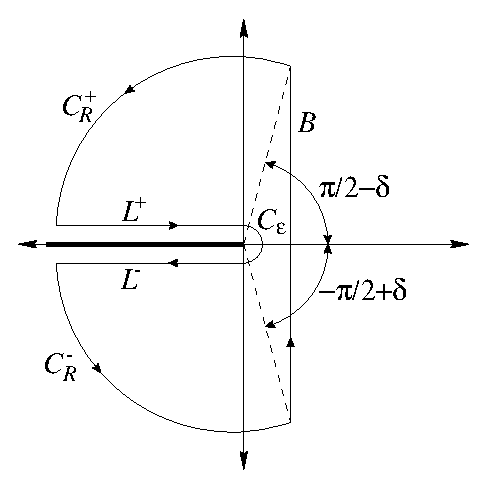
\includegraphics[width=0.4\textwidth]{ode/laplace/sqrts}
    \end{center}
    \caption{The path of integration.}
    \label{pi_over_sqrt_s}
  \end{figure}

  Since there are no residues inside the contour, we have
  \[
  \frac{1}{\imath 2 \pi} \left( \int_B + \int_{C_R^+} + \int_{L^+}
    + \int_{C_\epsilon} + \int_{L^-} + \int_{C_R^-} \right)
  \e^{s t} \left( \frac{\pi}{s} \right)^{1/2} \e^{-2 (a s)^{1/2}} \,\dd s = 0.
  \]
  We will evaluate the inverse Laplace transform for $t>0$.


  First we will show that the integral along
  $C_R^+$ vanishes as $R \to \infty$.  We parametrize the path of integration
  with $s = R \e^{\imath \theta}$ and write the integral along $C_R^+$ as the sum
  of two integrals.
  \[
  \int_{C_R^+} \cdots \,\dd s = \int_{\pi/2-\delta}^{\pi/2} \cdots \,\dd \theta + \int_{\pi/2}^\pi \cdots \,\dd \theta
  \]
  The first integral vanishes by the maximum modulus bound.  
  Note that the length of the path of integration is less than $2 \alpha$.
  \begin{align*}
    \left| \int_{\pi/2-\delta}^{\pi/2} \cdots \,\dd \theta \right|
    &\leq \left( \max_{\theta \in [\pi/2-\delta \ldots \pi/2]}
      \left| \e^{s t} \left( \frac{\pi}{s} \right)^{1/2} \e^{-2 (a s)^{1/2}}
      \right| \right) (2 \alpha) \\
    &= \e^{\alpha t} \frac{\sqrt{\pi}}{\sqrt{R}} (2 \alpha) \\
    &\to 0\ \mathrm{as}\ R \to \infty
  \end{align*}
  The second integral vanishes by Jordan's Lemma.
  \begin{align*}
    \left| \int_{\pi/2}^\pi \e^{R \e^{\imath \theta} t} 
      \frac{\sqrt{\pi}}{\sqrt{R \e^{\imath \theta}}}
      \e^{-2 \sqrt{a R \e^{\imath \theta} } } \,\dd \theta \right| 
    &\leq \int_{\pi/2}^\pi \left| \e^{R \e^{\imath \theta} t} 
      \frac{\sqrt{\pi}}{\sqrt{R \e^{\imath \theta}}}
      \e^{-2 \sqrt{a} \sqrt{R} \e^{\imath \theta/2} } \right| \,\dd \theta\\
    &\leq \frac{\sqrt{\pi}}{\sqrt{R}} \int_{\pi/2}^\pi \e^{R \cos(\theta) t} \,\dd \theta \\
    &\leq \frac{\sqrt{\pi}}{\sqrt{R}} \int_0^{\pi/2} \e^{- R t \sin(\phi)} \,\dd \phi \\
    &< \frac{\sqrt{\pi}}{\sqrt{R}} \frac{\pi}{2 R t} \\
    &\to 0\ \mathrm{as}\ R \to \infty
  \end{align*}
  We could show that the integral along $C_R^-$ vanishes by the same method.

  Now we have
  \[
  \frac{1}{\imath 2 \pi} \left( \int_B + \int_{L^+} + \int_{C_\epsilon} + \int_{L^-} \right)
  \e^{s t} \left( \frac{\pi}{s} \right)^{1/2} \e^{-2 (a s)^{1/2} } \,\dd s = 0.
  \]
  We show that the integral along $C_\epsilon$ vanishes as
  $\epsilon \to 0$ with the maximum modulus bound.  
  \begin{align*}
    \left| \int_{C_\epsilon} \e^{s t} \left( \frac{\pi}{s} \right)^{1/2} \e^{-2 (a s)^{1/2}}
      \,\dd s \right|
    &\leq \left(\max_{s \in C_\epsilon} \left| 
        \e^{s t} \left( \frac{\pi}{s} \right)^{1/2} \e^{-2 (a s)^{1/2}}
      \right| \right) (\pi \epsilon) \\
    &\leq \e^{\epsilon t} \frac{\sqrt{\pi}}{\sqrt{\epsilon}} \pi \epsilon\\
    &\to 0 \quad \mathrm{as}\ \epsilon \to 0.
  \end{align*}



  Now we can express the inverse Laplace transform in terms of the integrals
  along $L^+$ and $L^-$
  \begin{align*}
    f(t) &\equiv \frac{1}{\imath 2 \pi} \int_{\alpha - \imath \infty}^{\alpha + \imath \infty}
    \e^{s t} \left( \frac{\pi}{s} \right)^{1/2} \e^{-2 (a s)^{1/2}} \,\dd s\\
    &= - \frac{1}{\imath 2 \pi}\int_{L^+} 
    \e^{s t} \left( \frac{\pi}{s} \right)^{1/2} \e^{-2 (a s)^{1/2}} \,\dd s
    - \frac{1}{\imath 2 \pi}\int_{L^-} 
    \e^{s t} \left( \frac{\pi}{s} \right)^{1/2} \e^{-2 (a s)^{1/2}} \,\dd s.
  \end{align*}
  On $L^+$, $s = r \e^{\imath \pi}$, $\dd s = \e^{\imath \pi} \dd r = - \dd r$;
  on $L^-$, $s = r \e^{-\imath \pi}$, $\dd s = \e^{-\imath \pi} \dd r = - \dd r$.
  We can combine the integrals along the top and bottom of the branch cut.
  \begin{align*}
    f(t)
    &= - \frac{1}{\imath 2 \pi}\int_{\infty}^0
    \e^{-r t} \frac{\sqrt{\pi}}{\imath \sqrt{r}} \e^{- \imath 2 \sqrt{a} \sqrt{r}} (-\,\dd r)
    - \frac{1}{\imath 2 \pi}\int_{0}^{\infty} \e^{-r t} \frac{\sqrt{\pi}}{-\imath \sqrt{r}} 
    \e^{\imath 2 \sqrt{a} \sqrt{r}} (-\,\dd r) \\
    &= \frac{1}{2 \sqrt{\pi}} \int_0^\infty \e^{-r t} \frac{1}{\sqrt{r}} 
    \left( \e^{- \imath 2 \sqrt{a} \sqrt{r}} + \e^{\imath 2 \sqrt{a} \sqrt{r}} \right) \,\dd r \\
    &= \frac{1}{2 \sqrt{\pi}} \int_0^\infty \frac{1}{\sqrt{r}} \e^{-r t}
    2 \cos \left( 2 \sqrt{a} \sqrt{r} \right) \,\dd r \\
    \intertext{We make the change of variables $x = \sqrt{r}$.}
    &= \frac{1}{\sqrt{\pi}} \int_0^\infty \frac{1}{x} \e^{-t x^2}
    \cos \left( 2 \sqrt{a} x \right) 2 x\,\dd x \\
    &= \frac{2}{\sqrt{\pi}} \int_0^\infty \e^{-t x^2}
    \cos \left( 2 \sqrt{a} x \right) \,\dd x \\
    &= \frac{2}{\sqrt{\pi}} \sqrt{ \frac{ \pi }{ 4 t } }
    \e^{- 4 a / (4 t)} \\
    &= \frac{ \e^{-a / t} }{ \sqrt{t} }
  \end{align*}

  Thus the inverse Laplace transform is 
  \[
  \boxed{
    f(t) = \frac{ \e^{-a / t} }{ \sqrt{t} }
    }
  \]
\end{Solution}







%% \frac{d^4 y}{d t^4} - y = t
\begin{Solution}
  \label{solution y''''-y=t}
  We consider the problem
  \[
  \frac{\dd^4 y}{\dd t^4} - y = t, \qquad
  y(0) = y'(0) = y''(0) = y'''(0) = 0.
  \]
  We take the Laplace transform of the differential equation.
  \begin{gather*}
    s^4 \hat{y}(s) - s^3 y(0) - s^2 y'(0) - s y''(0) - y'''(0) - \hat{y}(s)
    = \frac{1}{s^2} \\
    s^4 \hat{y}(s) - \hat{y}(s) = \frac{1}{s^2} \\
    \hat{y}(s) = \frac{1}{s^2 (s^4 - 1)}
  \end{gather*}
  There are several ways in which we could carry out the inverse Laplace
  transform to find $y(t)$.  We could expand the right side in
  partial fractions and then use a table of Laplace transforms.
  Since the function is analytic except for isolated singularities and
  vanishes as $s \to \infty$ we could use the result,
  \[
  \mathcal{L}^{-1} [\hat{f}(s)]
  = \sum_{n = 1}^N \Res \left( \e^{s t} \hat{f}(s), s_n \right),
  \]
  where $\{s_k\}_{k=1}^n$ are the singularities of $\hat{f}(s)$.
  Since we can write the function as a product of simpler terms we could also
  apply the convolution theorem.

  We will first do the inverse Laplace transform by expanding the function 
  in partial fractions to obtain simpler rational functions.
  \begin{align*}
    \frac{1}{ s^2 (s^4 - 1) }
    &= \frac{1}{ s^2 (s - 1) (s + 1) (s - \imath) (s + \imath) } \\
    &= \frac{a}{s^2} + \frac{b}{s}
    + \frac{c}{ s - 1 } + \frac{d}{ s + 1 }
    + \frac{e}{ s - \imath } + \frac{f}{ s + \imath }
  \end{align*}
  \begin{align*}
    a &= \left[ \frac{1}{s^4 - 1} \right]_{s = 0} = -1 \\
    b &= \left[ \frac{\dd}{\dd s} \frac{1}{s^4 - 1} \right]_{s = 0} = 0 \\
    c &= \left[ \frac{1}{ s^2 (s + 1) (s - \imath) (s + \imath) }
    \right]_{s = 1} = \frac{1}{4} \\
    d &= \left[ \frac{1}{ s^2 (s - 1) (s - \imath) (s + \imath) }
    \right]_{s = -1} = - \frac{1}{4} \\
    e &= \left[ \frac{1}{ s^2 (s - 1) (s + 1) (s + \imath) }
    \right]_{s = \imath} = -\imath \frac{1}{4} \\
    f &= \left[ \frac{1}{ s^2 (s - 1) (s + 1) (s - \imath) }
    \right]_{s = -\imath} = \imath \frac{1}{4}
  \end{align*}
  Now we have simple functions that we can look up in a table.
  \begin{gather*}
    \hat{y}(s) = - \frac{1}{s^2} + \frac{1/4}{s-1} - \frac{1/4}{s+1}
    + \frac{1/2}{s^2 + 1} \\
    y(t) = \left( - t + \frac{1}{4} \e^t - \frac{1}{4} \e^{-t} + \frac{1}{2} \sin t
    \right) H(t) \\
    \boxed{
      y(t) = \left( - t + \frac{1}{2} \left( \sinh t + \sin t \right)
      \right) H(t)
      }
  \end{gather*}



  We can also do the inversion with the convolution theorem.
  \[
  \frac{1}{s^2 (s^4 - 1)} = \frac{1}{s^2} \frac{1}{s^2 + 1} \frac{1}{s^2-1}
  \]
  From a table of Laplace transforms we know,
  \begin{align*}
    \mathcal{L}^{-1} \left[ \frac{1}{s^2} \right] &= t, \\
    \mathcal{L}^{-1} \left[ \frac{1}{s^2 + 1} \right] &= \sin t, \\
    \mathcal{L}^{-1} \left[ \frac{1}{s^2 - 1} \right] &= \sinh t.
  \end{align*}
  Now we use the convolution theorem to find the solution for $t > 0$.
  \begin{align*}
    \mathcal{L}^{-1} \left[ \frac{1}{s^4 - 1} \right]
    &= \int_0^t \sinh(\tau) \sin(t-\tau) \,\dd \tau \\
    &= \frac{1}{2} \left( \sinh t - \sin t \right)
  \end{align*}
  \begin{align*}
    \mathcal{L}^{-1} \left[ \frac{1}{s^2 (s^4 - 1)} \right]
    &= \int_0^t \frac{1}{2} \left( \sinh \tau - \sin \tau \right)(t - \tau) \,\dd \tau \\
    &= - t + \frac{1}{2} \left( \sinh t + \sin t \right)
  \end{align*}
\end{Solution}







%% \frac{\dd y}{\dd t} = \sin t + \int_0^t y(\tau) \cos(t - \tau) \,\dd \tau
\begin{Solution}
  \label{solution y'=sin t int y cos}
  \begin{gather*}
    \frac{\dd y}{\dd t} = \sin t + \int_0^t y(\tau) \cos(t - \tau) \,\dd \tau \\
    s \hat{y}(s) - y(0) = \frac{1}{s^2 + 1} + \hat{y}(s) \frac{s}{s^2+1} \\
    (s^3 + s) \hat{y}(s) - s \hat{y}(s) = 1 \\
    \hat{y}(s) = \frac{1}{s^3} \\
    \boxed{
      y(t) = \frac{t^2}{2}
      }
  \end{gather*}
\end{Solution}







%% \frac{\dd u}{\dd t} + u(t) - u(t-1) = 0, \quad t \geq 0
\begin{Solution}
  \label{solution u'+u-u(t-1)=0}
  The Laplace transform of $u(t-1)$ is
  \begin{align*}
    \mathcal{L}[u(t-1)]
    &= \int_0^\infty \e^{-s t} u(t-1) \,\dd t \\
    &= \int_{-1}^\infty \e^{-s (t + 1)} u(t) \,\dd t \\
    &= \e^{-s} \int_{-1}^0 \e^{-s t} u(t) \,\dd t + \e^{-s} \int_0^\infty \e^{-s t} u(t) \,\dd t \\
    &= \e^{-s} \int_{-1}^0 \e^{-s t} u_0(t) \,\dd t + \e^{-s} \hat{u}(s).
  \end{align*}

  We take the Laplace transform of the difference-differential equation.
  \begin{gather*}
    s \hat{u}(s) - u(0) + \hat{u}(s) - \e^{-s} \int_{-1}^0 \e^{-s t} u_0(t) \,\dd t
    + \e^{-s} \hat{u}(s) = 0 \\
    (1 + s - \e^{-s} ) \hat{u}(s) = u_0(0) + \e^{-s} \int_{-1}^0 \e^{-s t} u_0(t) \,\dd t \\
    \boxed{
      \hat{u}(s) = \frac{ u_0(0) }{ 1 + s - \e^{-s} } 
      + \frac{ \e^{-s} }{ 1 + s - \e^{-s} } \int_{-1}^0 \e^{-s t} u_0(t) \,\dd t
      }
  \end{gather*}

  Consider the case  $u_0(t) = 1$.
  \begin{gather*}
    \hat{u}(s) = \frac{ 1 }{ 1 + s - \e^{-s} } 
    + \frac{ \e^{-s} }{ 1 + s - \e^{-s} } \int_{-1}^0 \e^{-s t} \,\dd t \\
    \hat{u}(s) = \frac{ 1 }{ 1 + s - \e^{-s} } + \frac{ \e^{-s} }{ 1 + s - \e^{-s} } 
    \left( - \frac{1}{s} + \frac{1}{s} \e^s \right) \\
    \hat{u}(s) = \frac{ 1/s + 1 - \e^{-s} / s }{ 1 + s - \e^{-s} } \\
    \hat{u}(s) = \frac{1}{s} \\
    \boxed{
      u(t) = 1
      }
  \end{gather*}
  Clearly this solution satisfies the difference-differential equation.
\end{Solution}







%% \frac{\dd^2 y}{\dd t^2} - y = f(t); \qquad y(0) = 1, \quad \frac{\dd y}{\dd t}(0) = 0.
\begin{Solution}
  \label{solution f(t)=1,0<t<pi}
  We consider the problem,
  \[
  \frac{\dd^2 y}{\dd t^2} - y = f(t), \quad y(0) = 1, \quad y'(0) = 0,
  \]
  where $f(t)$ is periodic with period $2 \pi$ and is defined by,
  \[
  f(t) = 
  \begin{cases}
    1 & 0 \leq t < \pi, \\
    0 & \pi \leq t < 2\pi.
  \end{cases}
  \]

  We take the Laplace transform of the differential equation.
  \begin{gather*}
    s^2 \hat{y}(s) - s y(0) - y'(0) - \hat{y}(s) = \hat{f}(s) \\
    s^2 \hat{y}(s) - s - \hat{y}(s) = \hat{f}(s) \\
    \hat{y}(s) = \frac{s}{s^2 - 1} + \frac{ \hat{f}(s) }{s^2 - 1}
  \end{gather*}
  By inspection, (of a table of Laplace transforms), we see that
  \begin{gather*}
    \mathcal{L}^{-1} \left[ \frac{s}{s^2 - 1} \right] = \cosh(t) H(t), \\
    \mathcal{L}^{-1} \left[ \frac{1}{s^2 - 1} \right] = \sinh(t) H(t).
  \end{gather*}
  Now we use the convolution theorem.
  \begin{align*}
    \mathcal{L}^{-1} \left[ \frac{ \hat{f}(s) }{ s^2  - 1 } \right]
    &= \int_0^t f(\tau) \sinh(t - \tau) \,\dd \tau \\
  \end{align*}
  The solution for positive $t$ is
  \[
  \boxed{
    y(t) = \cosh(t) + \int_0^t f(\tau) \sinh(t - \tau) \,\dd \tau. 
    }
  \]
  Clearly the solution is continuous because the integral of a bounded function
  is continuous.  The first derivative of the solution is
  \begin{gather*}
    y'(t) = \sinh t + f(t) \sinh(0) + \int_0^t f(\tau) \cosh(t - \tau) \,\dd \tau \\
    y'(t) = \sinh t + \int_0^t f(\tau) \cosh(t - \tau) \,\dd \tau 
  \end{gather*}
  We see that the first derivative is also continuous.
\end{Solution}











\begin{Solution}
  \label{solution y' + int y = e-t}
  We consider the problem
  \[
  \frac{\dd y}{\dd t} + \int_0^t y(\tau) \,\dd \tau = \e^{-t},\quad y(0) = 1.
  \]
  We take the Laplace transform of the equation and solve for $\hat{y}$.
  \begin{gather*}
    s \hat{y} - y(0) + \frac{\hat{y}}{s} = \frac{1}{s + 1} \\
    \hat{y} = \frac{ s (s + 2) }{ (s + 1)(s^2 + 1) }
  \end{gather*}
  We expand the right side in partial fractions.
  \[
  \hat{y} = - \frac{1}{2(s + 1)} + \frac{1 + 3 s}{2 (s^2 + 1)}
  \]
  We use a table of Laplace transforms to do the inversion.
  \[
  \boxed{
    y = - \frac{1}{2} \e^{-t} + \frac{1}{2} ( \sin(t) + 3 \cos(t) )
    }
  \]
\end{Solution}






%% CONTINUE CHECK
\begin{Solution}
  \label{solution circuit i1 i2 q}
  We consider the problem
  \begin{gather*}
    L \frac{\dd i_1}{\dd t} + R i_1 + q / C = E_0\\
    L \frac{\dd i_2}{\dd t} + R i_2 - q / C = 0\\
    \frac{\dd q}{\dd t} = i_1 - i_2 \\
    i_1(0)=i_2(0)=\frac{E_0}{2R},\quad q(0) = 0.
  \end{gather*}
  We take the Laplace transform of the system of differential equations.
  \begin{gather*}
    L \left( s \hat{i}_1 - \frac{E_0}{2 R} \right) + R \hat{i}_1 
    + \frac{ \hat{q} }{C} = \frac{E_0}{s} \\
    L \left( s \hat{i}_2 - \frac{E_0}{2 R} \right) + R \hat{i}_2 
    - \frac{ \hat{q} }{C} = 0 \\
    s \hat{q} = \hat{i}_1 - \hat{i}_2
  \end{gather*}
  We solve for $\hat{i}_1$, $\hat{i}_2$ and $\hat{q}$.
  \begin{gather*}
    \hat{i}_1 = \frac{E_0}{2} \left( \frac{1}{R s} 
      + \frac{1/L}{ s^2 + R s / L + 2 / (C L) } \right) \\
    \hat{i}_2 = \frac{E_0}{2} \left( \frac{1}{R s} 
      - \frac{1/L}{ s^2 + R s / L + 2 / (C L) } \right) \\
    \hat{q} = \frac{C E_0}{2} \left( \frac{1}{s}
      - \frac{ s + R/L }{ s^2 + R s / L + 2 / (C L) } \right)
  \end{gather*}
  We factor the polynomials in the denominators.
  \begin{gather*}
    \hat{i}_1 = \frac{E_0}{2} \left( \frac{1}{R s} 
      + \frac{1/L}{ (s + \alpha - \imath \omega)(s + \alpha + \imath \omega) } \right) \\
    \hat{i}_2 = \frac{E_0}{2} \left( \frac{1}{R s} 
      - \frac{1/L}{ (s + \alpha - \imath \omega)(s + \alpha + \imath \omega) } \right) \\
    \hat{q} = \frac{C E_0}{2} \left( \frac{1}{s}
      - \frac{ s + 2 \alpha }{ (s + \alpha - \imath \omega)(s + \alpha + \imath \omega) } \right)
  \end{gather*}
  Here we have defined
  \[
  \alpha = \frac{R}{2L} \quad \mathrm{and} \quad \omega^2 = \frac{2}{LC} - \alpha^2.
  \]
  We expand the functions in partial fractions.
  \begin{gather*}
    \hat{i}_1 = \frac{E_0}{2} \left( \frac{1}{R s} 
      + \frac{\imath}{2 \omega L} \left( 
        \frac{1}{s + \alpha + \imath \omega} - \frac{1}{s + \alpha - \imath \omega} \right) \right) \\
    \hat{i}_2 = \frac{E_0}{2} \left( \frac{1}{R s} 
      - \frac{\imath}{2 \omega L} \left( 
        \frac{1}{s + \alpha + \imath \omega} - \frac{1}{s + \alpha - \imath \omega} \right) \right) \\
    \hat{q} = \frac{C E_0}{2} \left( \frac{1}{s}
      + \frac{\imath}{2 \omega} \left( 
        \frac{ \alpha + \imath \omega }{ s + \alpha - \imath \omega }
        - \frac{ \alpha - \imath \omega }{ s + \alpha + \imath \omega } \right) \right)
  \end{gather*}
  Now we can do the inversion with a table of Laplace transforms.
  \begin{gather*}
    i_1 = \frac{E_0}{2} \left( \frac{1}{R} 
      + \frac{\imath}{2 \omega L} \left( \e^{(-\alpha - \imath \omega) t} - \e^{(-\alpha + \imath \omega) t} \right) \right) \\
    i_2 = \frac{E_0}{2} \left( \frac{1}{R} 
      - \frac{\imath}{2 \omega L} \left( \e^{(-\alpha - \imath \omega) t} - \e^{(-\alpha + \imath \omega) t} \right) \right) \\
    q = \frac{C E_0}{2} \left( 1
      + \frac{\imath}{2 \omega} \left( 
        (\alpha + \imath \omega) \e^{(-\alpha + \imath \omega) t}
        - (\alpha - \imath \omega) \e^{(-\alpha - \imath \omega) t} \right) \right)
  \end{gather*}
  We simplify the expressions to obtain the solutions.
  \begin{gather*}
    i_1 = \frac{E_0}{2} \left( \frac{1}{R} 
      + \frac{1}{\omega L} \e^{-\alpha t} \sin(\omega t) \right) \\
    i_2 = \frac{E_0}{2} \left( \frac{1}{R} 
      - \frac{1}{\omega L} \e^{-\alpha t} \sin(\omega t) \right) \\
    q = \frac{C E_0}{2} \left( 1
      - \e^{-\alpha t} \left( \cos(\omega t) + \frac{\alpha}{\omega} \sin(\omega t) \right) \right)
  \end{gather*}
\end{Solution}







\begin{Solution}
  \label{solution y4y4y=4e-t}
    We consider the problem
  \[
  y''+ 4 y' + 4 y = 4 \e^{-t}, \quad y(0) = 2,~y'(0) = -3
  \]
  We take the Laplace transform of the differential equation
  and solve for $\hat{y}(s)$.
  \begin{gather*}
    s^2 \hat{y} - s y(0) - y'(0) + 4 s \hat{y} - 4 y(0) + 4 \hat{y} 
    = \frac{4}{s + 1}
    \\
    s^2 \hat{y} - 2 s + 3 + 4 s \hat{y} - 8 + 4 \hat{y} = \frac{4}{s + 1}
    \\
    \hat{y} = \frac{4}{(s + 1)(s + 2)^2} + \frac{2 s + 5}{(s + 2)^2}
    \\
    \hat{y} = \frac{4}{s + 1} - \frac{2}{s + 2} - \frac{3}{(s + 2)^2}
  \end{gather*}
  We take the inverse Laplace transform to determine the solution.
  \[
  \boxed{
    y = 4 \e^{-t} - ( 2 + 3 t) \e^{-2 t}
    }
  \]
\end{Solution}








\raggedbottom
}
